\documentclass[letterpaper]{article}
\usepackage{calc,amsmath,amssymb,amsfonts}
\usepackage[T1]{fontenc}
\usepackage[english]{babel}
\usepackage{xcolor,longfbox,fancyhdr}
\usepackage[top=1in,bottom=0.5in,hmargin=1in,nohead,includefoot,foot=0.5in,footskip=0.9602in]{geometry}
\usepackage{array,supertabular,hhline,enumitem,hyperref}
\hypersetup{colorlinks=true,allcolors=blue,pdftitle=Machine Learning - Driver Drowsiness Detection,pdfauthor=Nafe Muhtasim}
\usepackage[pdftex]{graphicx}
\makeatletter\newdimen\@tempdimd\makeatother
% Outline numbering
\setcounter{secnumdepth}{0}
% Text styles
\newcommand\textstyleHeadingiiiChar[1]{\textrm{\textcolor[HTML]{1F3763}{#1}}}
\newcommand\textstyleListLabelx[1]{\textrm{#1}}
\newcommand\textstyleInternetlink[1]{\textcolor[HTML]{0563C1}{#1}}
\newcommand\textstyleHeadingiiChar[1]{\textrm{\textcolor[HTML]{2F5496}{#1}}}
\makeatletter
\newcommand\arraybslash{\let\\\@arraycr}
\makeatother
% Pages
\fancypagestyle{Standard}{\fancyhf{}
  \fancyhead[L]{}
  \fancyfoot[R]{\thepage{}\ {\textbar} Page}
  \renewcommand\headrulewidth{0pt}
  \renewcommand\footrulewidth{0pt}
  \renewcommand\thepage{\arabic{page}}
}
\fancypagestyle{FirstPage}{\fancyhf{}
  \fancyhead[L]{}
  \fancyfoot[L]{}
  \renewcommand\headrulewidth{0pt}
  \renewcommand\footrulewidth{0pt}
  \renewcommand\thepage{\arabic{page}}
}
\pagestyle{Standard}
\setlength\tabcolsep{1mm}
\renewcommand\arraystretch{1.3}
\title{Machine Learning - Driver Drowsiness Detection}
\author{Nafe Muhtasim}
\date{2024-12-20}
\begin{document}
\clearpage
\pagestyle{Standard}
\thispagestyle{FirstPage}

\bigskip



\begin{center}
\begin{longfbox}[margin-right=0.1299in,margin-left=0.1299in,margin-top=0mm,margin-bottom=0mm,border-style=none,padding=0mm,vertical-align=top,width=0.0161in]
\begin{center}
\tablefirsthead{}
\tablehead{}
\tabletail{}
\tablelasttail{}
\begin{supertabular}{m{1.8cm}}
\textcolor[HTML]{002060}{December 20, 2024}

~

~

~
\\
\end{supertabular}
\end{center}
\end{longfbox}
\end{center}
\begin{center}
\begin{longfbox}[margin-right=0.1299in,margin-left=0.1299in,margin-top=0mm,margin-bottom=0mm,border-style=none,padding=0mm,vertical-align=top,raise=-2.0008in,width=0.0161in]
\begin{center}
\tablefirsthead{}
\tablehead{}
\tabletail{}
\tablelasttail{}
\begin{supertabular}{|m{1.8cm}}
~
\\
\textcolor[HTML]{002060}{Machine Learning - Driver Drowsiness Detection}\\
\end{supertabular}
\end{center}
\end{longfbox}
\end{center}

\bigskip


\bigskip

\clearpage{\color[HTML]{2F5496}
Table of Contents}

\setcounter{tocdepth}{3}
\tableofcontents

\bigskip


\bigskip


\bigskip


\bigskip


\bigskip


\bigskip


\bigskip


\bigskip


\bigskip


\bigskip


\bigskip


\bigskip


\bigskip


\bigskip


\bigskip


\bigskip


\bigskip


\bigskip


\bigskip


\bigskip


\bigskip


\bigskip


\bigskip


\bigskip

\section[Data Source\ \ ]{\textbf{Data Source}\textcolor[HTML]{002060}{\ \ }}
\subsection{Dataset Description}
An open EEG dataset released in 2019 by Cao et al. was used in our study. The study involved 27 voluntary participants
aged 22–28 years, consisting of National Chiao Tung University students and staff. They participated in a 90-minute
sustained-attention driving task multiple times on the same or different days, resulting in 62 EEG datasets.
Participants were required to have normal or corrected-to-normal vision and no history of sleep deprivation, drug
abuse, or irregular sleep patterns prior to the experiments. They avoided alcohol, caffeine, and strenuous exercise a
day before the experiments. A VR driving environment was created using a dynamic driving simulator mounted on a
six-degree-of-freedom Stewart motion platform. Six interactive highway driving scenes synchronized over local area
networks were projected onto the screens at viewing angles of 0°, 42°, 84°, 180°, 276°, and 318° to provide a nearly
complete 360° visual field.  An event-related lane-departure paradigm3 was implemented in the VR-based driving
simulator using WorldToolKit (WTK) R9 Direct and Visual C++.  The driving task involved a visually monotonous night on
a straight four-lane highway that mirrors real-life driving conditions. The lane-departure paradigm measured
participants' reaction times to perturbations during a continuous driving task. Participants were instructed to keep
the car in the center of the lane and respond to random lane-departure events by steering the car back to the original
lane. The task lasted 90 minutes without breaks, and participants' activities were monitored via a surveillance video
camera.


\bigskip

\textbf{Reference Link: \ }\url{https://www.nature.com/articles/s41597-019-0027-4}


\bigskip

\centering
\lfbox[margin=0mm,border-style=none,padding=0mm,vertical-align=top]{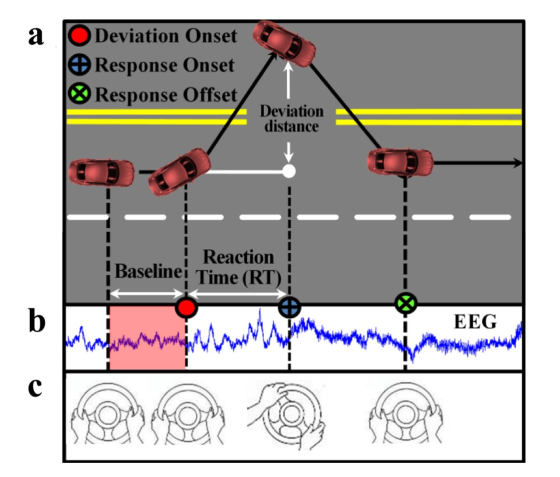
\includegraphics[width=4.402in,height=3.7492in]{a0000-img001.png}}
\par
\subsubsection[Figure: Experimental design.]{\textbf{Figure: }Experimental design.}
\begin{enumerate}[series=listWWNumiv,label=(\alph*),ref=\alph*]
\item {\centering
Event-related lane-deviation task. (b, c) Simultaneous EEG and behavioral recording.
\par}
\end{enumerate}

\bigskip

As shown in (Fig. a), lane-departure events were randomly induced to make the car drift from the original cruising lane
towards the left or right sides (deviation onset). Each participant was instructed to quickly compensate for this
perturbation by steering the wheel (response onset) to cause the car to move back to the original cruising lane
(response offset). To avoid the impacts of other factors during the task, participants only reacted to the
lane-perturbation event by turning the steering wheel. They did not have to control the accelerator or brake pedals in
this experiment. Each lane-departure event was defined as a “trial,” including a baseline period, deviation onset,
response onset, and response offset. EEG signals were recorded simultaneously (Fig. b).

The corresponding directions for turning the steering wheel are shown in (Fig. c.) Of note, the next trial occurred
within a 5–10 second interval after finishing the current trial, during which the subject had to maneuver the car back
to the center line of the third car lane. If the participant fell asleep during the experiment, no feedback was
provided to alert him/her.


\bigskip

\subsection{Electrode Layout in EEG Cap}
\centering
\lfbox[margin=0mm,border-style=none,padding=0mm,vertical-align=top]{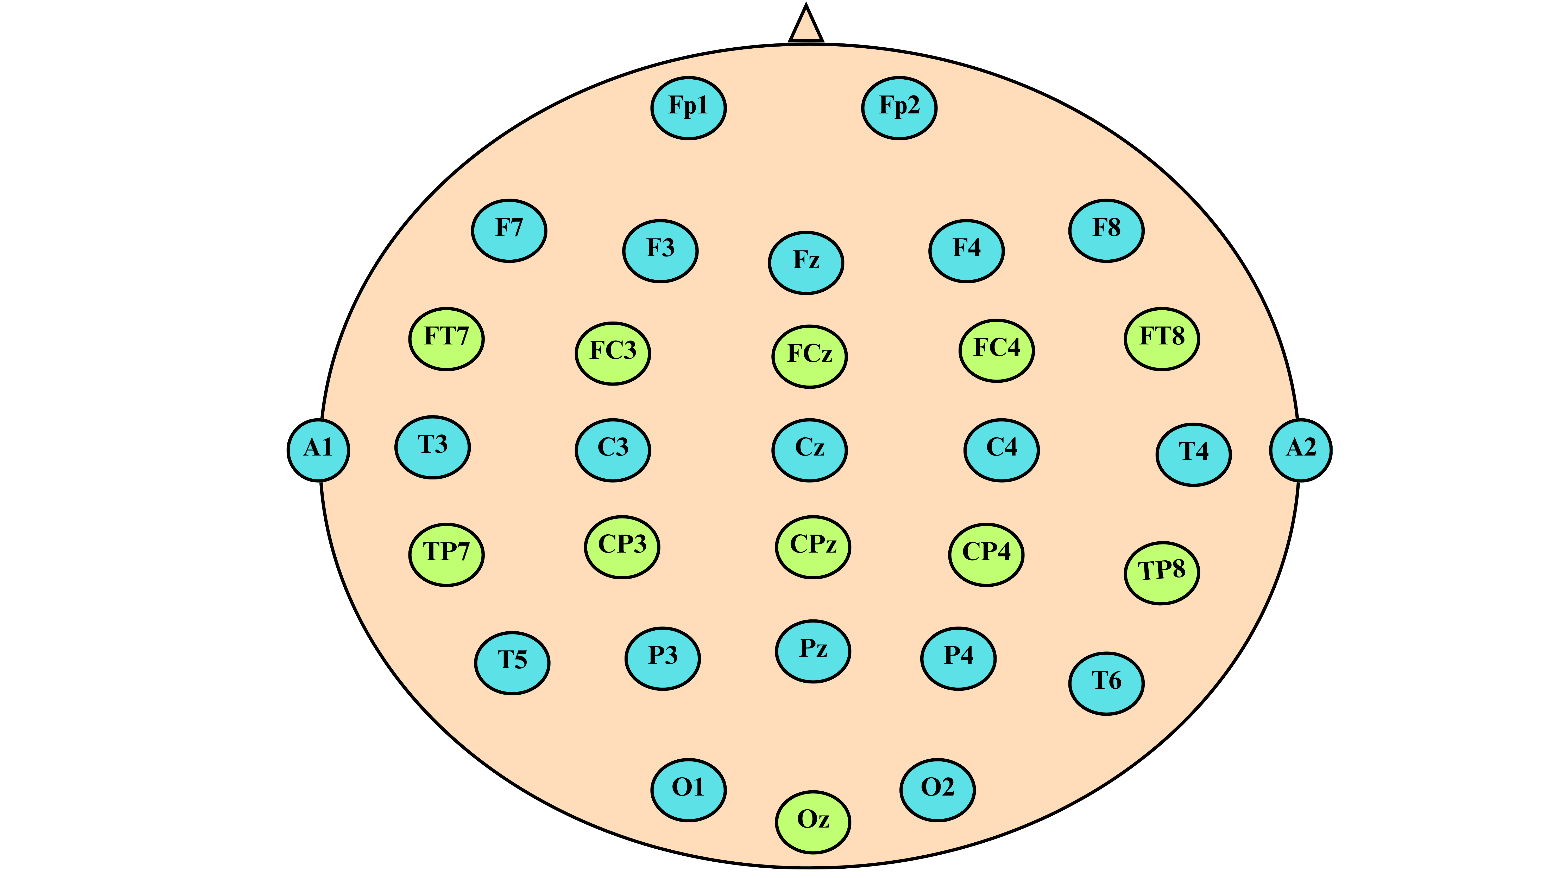
\includegraphics[width=4.0972in,height=3.198in]{a0000-img002.png}}
\par

\bigskip

\centering
\lfbox[margin=0mm,border-style=none,padding=0mm,vertical-align=top]{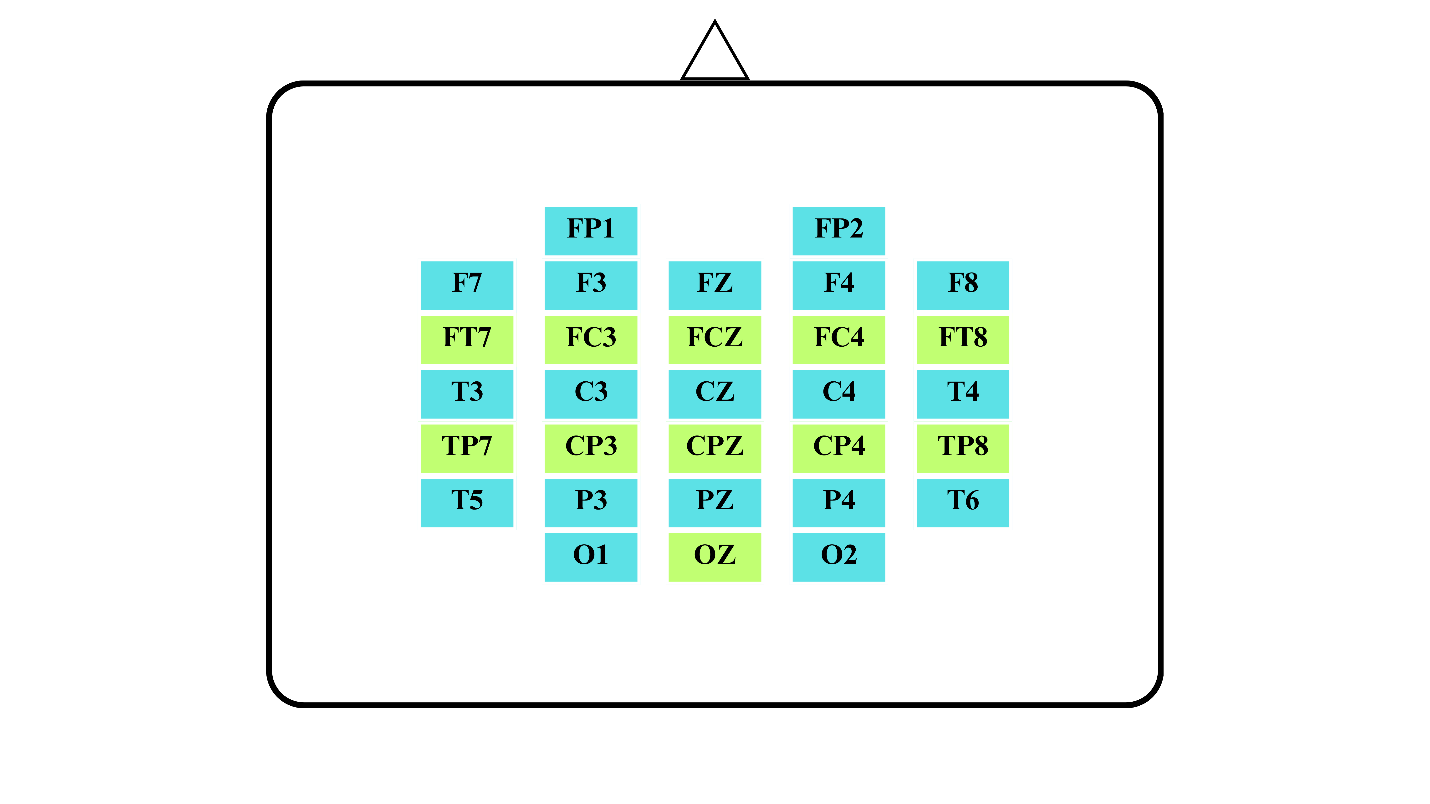
\includegraphics[width=6.5in,height=3.6563in]{a0000-img003.png}}
\par
\subsubsection[Figure: EEG Cap Electrode Layout. Blue electrodes represent the 10–20 system, and green indicates
additional electrodes. Contact impedance was maintained below 5 k$\Omega $ for all electrodes.]{\textbf{Figure:}
\textstyleHeadingiiiChar{EEG Cap Electrode Layout. Blue electrodes represent the 10–20 system, and green indicates
additional electrodes. Contact impedance was maintained below 5 k$\Omega $ for all electrodes.}}

\bigskip

\subsection{Data Recording and Storage}
EEG data were recorded using a Scan SynAmps2 Express system with 32 Ag/AgCl electrodes and were digitized at 500 Hz. The
stimulus computer recorded Vehicle trajectories and events in a log file, which synchronized triggers with the EEG
acquisition system. The data were integrated into a new file and imported into EEGLAB in MATLAB.

The EEG signals included 32 channels from electrodes placed according to a modified international 10–20 system. The
recordings were analyzed using the EEGLAB toolbox in MATLAB, and events were classified as deviation onset, response
onset, or response offset.

The first 32 signals were from the Fp1, Fp2, F7, F3, Fz, F4, F8, FT7, FC3, FCZ, FC4, FT8, T3, C3, Cz, C4, T4, TP7, CP3,
CPz, CP4, TP8, A1, T5, P3, PZ, P4, T6, A2, O1, Oz and O2 electrodes. Two electrodes (A1 and A2) were references placed
on the mastoid bones. The 33rd signal was used to describe the position of the simulated vehicle. A wired EEG cap with
30 EEG electrodes and two reference electrodes, placed according to a modified international 10–20 system, sampled the
EEG signals at 500 Hz throughout the experiment.


\bigskip


\bigskip


\bigskip


\bigskip

\subsection{Data extraction}
The dataset has already been preprocessed by its authors in the following steps:

\begin{itemize}[series=listWWNumv,label=\textstyleListLabelx{[F0B7?]}]
\item The raw EEG signals were filtered by 1-Hz high-pass and 50-Hz low-pass finite impulse response (FIR) filters.
\item For artifact rejection, apparent eye blink contamination was manually removed. Ocular and muscular artifacts were
removed using the Automatic Artifact Removal (AAR) plug-in provided in EEGLAB.
\item The original data was further down-sampled from 500 Hz to 128 Hz. 3s-long EEG samples were extracted prior to
deviation onset for each trial. 
\end{itemize}

\bigskip

\textbf{Reference Link:} \url{https://arxiv.org/abs/2106.00613}


\bigskip


\bigskip


\bigskip


\bigskip


\bigskip


\bigskip


\bigskip


\bigskip


\bigskip


\bigskip


\bigskip


\bigskip


\bigskip


\bigskip


\bigskip


\bigskip

\section[System Workflow]{\textbf{System Workflow}}
\centering
\lfbox[margin=0mm,border-style=none,padding=0mm,vertical-align=top]{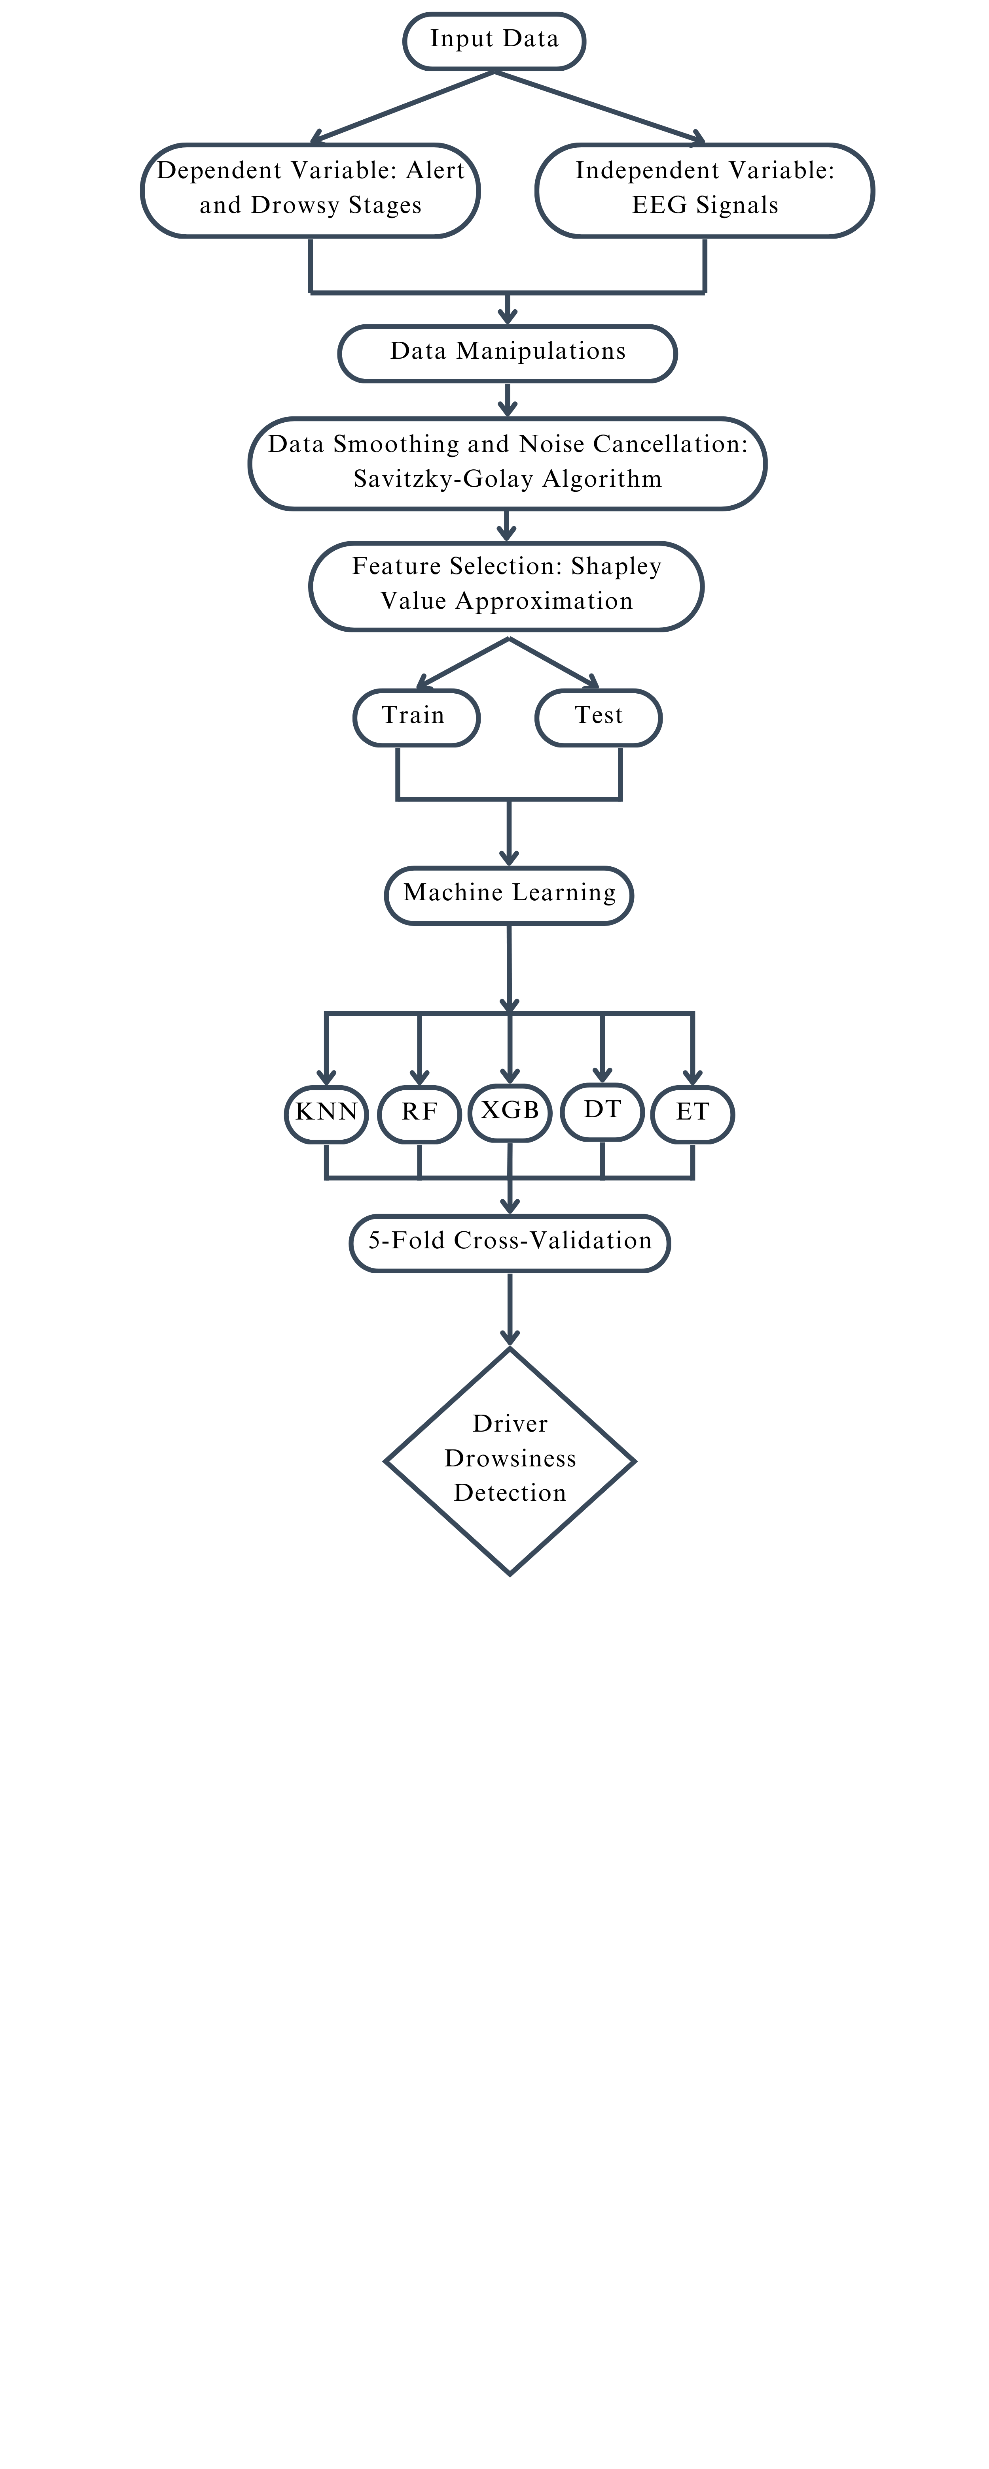
\includegraphics[width=3.5311in,height=7.2701in]{a0000-img004.png}}
\par

\bigskip

\subsubsection[Figure: System Workflow Diagram]{\textbf{Figure:} System Workflow Diagram}

\bigskip


\bigskip


\bigskip

\section[Scattered Machine Learning]{\textbf{Scattered Machine Learning}}

\bigskip


\bigskip

\subsection{Accuracy Metrics Table}
\begin{flushleft}
\tablefirsthead{}
\tablehead{}
\tabletail{}
\tablelasttail{}
\begin{supertabular}{|m{0.7677598in}|m{0.41085985in}|m{1.0830599in}|m{0.66565984in}|m{0.9497598in}|m{0.8309598in}|}
\hline
{\bfseries Feature} &
{\bfseries KNN} &
{\bfseries Random Forest} &
{\bfseries XGBoost} &
{\bfseries Decision Tree} &
{\bfseries Extra Trees}\\\hline
{\bfseries Feature 5} &
0.58 &
0.61 &
0.61 &
0.55 &
0.61\\\hline
{\bfseries Feature 8} &
0.61 &
0.65 &
0.65 &
0.57 &
0.64\\\hline
{\bfseries Feature 16} &
0.68 &
0.70 &
0.71 &
0.60 &
0.69\\\hline
{\bfseries Feature 22} &
0.69 &
0.71 &
0.72 &
0.60 &
0.69\\\hline
{\bfseries Feature 30} &
0.70 &
0.71 &
0.73 &
0.61 &
0.69\\\hline
\end{supertabular}
\end{flushleft}

\bigskip

\subsection{Precision Metrics Table}
\begin{flushleft}
\tablefirsthead{}
\tablehead{}
\tabletail{}
\tablelasttail{}
\begin{supertabular}{|m{0.7677598in}|m{0.41085985in}|m{1.0830599in}|m{0.66565984in}|m{0.9497598in}|m{0.8309598in}|}
\hline
{\bfseries Feature} &
{\bfseries KNN} &
{\bfseries Random Forest} &
{\bfseries XGBoost} &
{\bfseries Decision Tree} &
{\bfseries Extra Trees}\\\hline
{\bfseries Feature 5} &
0.58 &
0.61 &
0.62 &
0.55 &
0.61\\\hline
{\bfseries Feature 8} &
0.61 &
0.65 &
0.65 &
0.57 &
0.65\\\hline
{\bfseries Feature 16} &
0.69 &
0.72 &
0.72 &
0.60 &
0.71\\\hline
{\bfseries Feature 22} &
0.71 &
0.73 &
0.74 &
0.60 &
0.72\\\hline
{\bfseries Feature 30} &
0.71 &
0.73 &
0.75 &
0.61 &
0.72\\\hline
\end{supertabular}
\end{flushleft}

\bigskip

\subsection{Recall Metrics Table}
\begin{flushleft}
\tablefirsthead{}
\tablehead{}
\tabletail{}
\tablelasttail{}
\begin{supertabular}{|m{0.7677598in}|m{0.41085985in}|m{1.0830599in}|m{0.66565984in}|m{0.9497598in}|m{0.8309598in}|}
\hline
{\bfseries Feature} &
{\bfseries KNN} &
{\bfseries Random Forest} &
{\bfseries XGBoost} &
{\bfseries Decision Tree} &
{\bfseries Extra Trees}\\\hline
{\bfseries Feature 5} &
0.57 &
0.60 &
0.59 &
0.55 &
0.57\\\hline
{\bfseries Feature 8} &
0.61 &
0.63 &
0.64 &
0.57 &
0.60\\\hline
{\bfseries Feature 16} &
0.65 &
0.65 &
0.68 &
0.60 &
0.63\\\hline
{\bfseries Feature 22} &
0.65 &
0.66 &
0.70 &
0.60 &
0.63\\\hline
{\bfseries Feature 30} &
0.66 &
0.66 &
0.71 &
0.60 &
0.63\\\hline
\end{supertabular}
\end{flushleft}

\bigskip


\bigskip


\bigskip

\subsection[F1{}-score Metrics Table]{F1-score Metrics Table}
\begin{flushleft}
\tablefirsthead{}
\tablehead{}
\tabletail{}
\tablelasttail{}
\begin{supertabular}{|m{0.7677598in}|m{0.41085985in}|m{1.0830599in}|m{0.66565984in}|m{0.9497598in}|m{0.8309598in}|}
\hline
{\bfseries Feature} &
{\bfseries KNN} &
{\bfseries Random Forest} &
{\bfseries XGBoost} &
{\bfseries Decision Tree} &
{\bfseries Extra Trees}\\\hline
{\bfseries Feature 5} &
0.57 &
0.60 &
0.61 &
0.55 &
0.59\\\hline
{\bfseries Feature 8} &
0.61 &
0.64 &
0.64 &
0.57 &
0.62\\\hline
{\bfseries Feature 16} &
0.67 &
0.68 &
0.70 &
0.60 &
0.67\\\hline
{\bfseries Feature 22} &
0.68 &
0.69 &
0.72 &
0.60 &
0.67\\\hline
{\bfseries Feature 30} &
0.68 &
0.69 &
0.73 &
0.60 &
0.67\\\hline
\end{supertabular}
\end{flushleft}

\bigskip

\subsection{Training Time (s) Metrics Table}
\begin{flushleft}
\tablefirsthead{}
\tablehead{}
\tabletail{}
\tablelasttail{}
\begin{supertabular}{|m{0.7677598in}|m{0.49135986in}|m{1.0830599in}|m{0.66565984in}|m{0.9497598in}|m{0.8309598in}|}
\hline
{\bfseries Feature} &
{\bfseries KNN} &
{\bfseries Random Forest} &
{\bfseries XGBoost} &
{\bfseries Decision Tree} &
{\bfseries Extra Trees}\\\hline
{\bfseries Feature 5} &
0.9037 &
774.2472 &
3.7172 &
25.1586 &
130.6855\\\hline
{\bfseries Feature 8} &
1.2688 &
790.3788 &
4.2159 &
40.8654 &
143.5649\\\hline
{\bfseries Feature 16} &
0.0310 &
1593.1800 &
5.0250 &
90.0796 &
211.1900\\\hline
{\bfseries Feature 22} &
0.0518 &
1636.6767 &
5.5533 &
125.3308 &
219.2712\\\hline
{\bfseries Feature 30} &
0.0319 &
2069.2782 &
6.7332 &
168.4359 &
251.6688\\\hline
\end{supertabular}
\end{flushleft}

\bigskip


\bigskip


\bigskip


\bigskip


\bigskip


\bigskip


\bigskip


\bigskip


\bigskip


\bigskip


\bigskip


\bigskip


\bigskip

\section[Data Manipulation]{\textbf{Data Manipulation}}

\bigskip

\subsection{Data Manipulation Methodology}
Segregation:

\begin{itemize}[series=listWWNumi,label=[F0B7?]]
\item The EEG samples are segregated into alert and drowsy states for all the subjects based on the 'substate' variable.
\item The segregated alert and drowsy data are saved into new '.mat' files.
\end{itemize}
Manipulating alert and drowsy state data:

\begin{itemize}[series=listWWNumii,label=[F0B7?]]
\item The alert data is loaded and transposed, concatenating all EEG samples into a new data frame.
\item Similar manipulation is performed on the drowsy state data.
\end{itemize}
Creating Combined Dataset:

\begin{itemize}[series=listWWNumiii,label=[F0B7?]]
\item The manipulated alert and drowsy datasets are concatenated row-wise into a new data frame.
\end{itemize}
\centering
\lfbox[margin=0mm,border-style=none,padding=0mm,vertical-align=top]{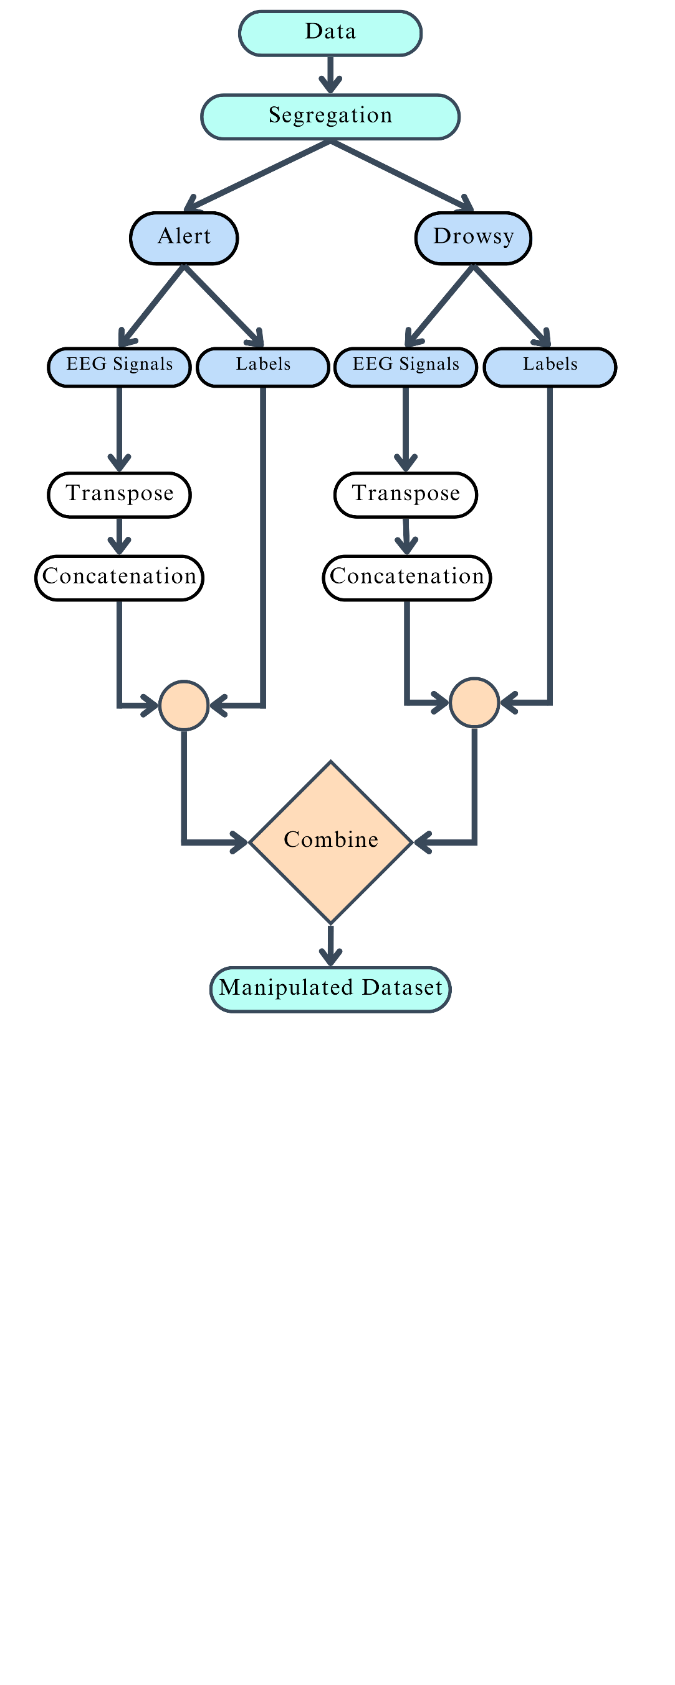
\includegraphics[width=3.0508in,height=4.778in]{a0000-img005.png}}
\par
\subsubsection[Figure: Flowchart of the Data Manipulation Methodology.]{\textbf{Figure: }Flowchart of the Data
Manipulation Methodology.}

\bigskip

\subsection{Data Manipulation Result}
Prior to manipulation, the initial EEG dataset contained 2022 samples, each with 30 channels and 384 data points,
recorded over 3 seconds at a sampling rate of 128Hz from 11 subjects. The shape of each alert and drowsy states dataset
was (1011, 384, 30) [1]. 

After manipulation, the dataset was transformed into a flat structure with 776448 rows and 31 columns where the
additional column represented the 'substate' variable, which contains alert (0) and drowsy (1) states. This
manipulation resulted in a new data frame for both alert and drowsy states, each with a shape of (388224, 31).


\bigskip


\bigskip


\lfbox[margin=0mm,border-style=none,padding=0mm,vertical-align=top]{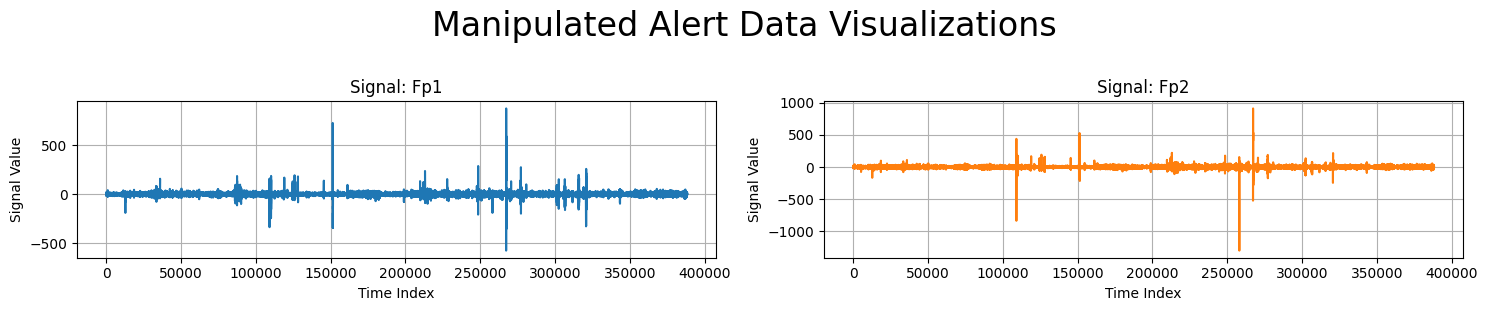
\includegraphics[width=6.5in,height=1.3591in]{a0000-img006.png}}



\lfbox[margin=0mm,border-style=none,padding=0mm,vertical-align=top]{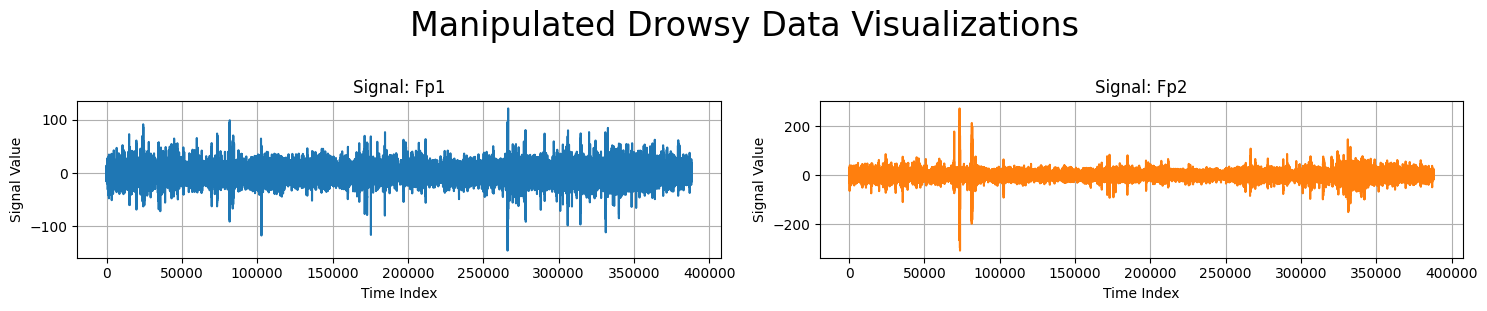
\includegraphics[width=6.5in,height=1.3591in]{a0000-img007.png}}



\bigskip

{\centering
\textbf{Figure:} Visualization of Manipulated Alert and Drowsy Data for Signal Fp1 and Fp2
\par}


\bigskip

\subsection{References}
[1]\ \ J. Cui \textit{et al.}, “A compact and interpretable convolutional neural network for cross-subject driver
drowsiness detection from single-channel EEG,” \textit{Methods}, vol. 202, pp. 173–184, Jun. 2022, doi:
10.1016/j.ymeth.2021.04.017.


\bigskip


\bigskip


\bigskip


\bigskip


\bigskip


\bigskip

\section[Noise Cancellation: Savitzky{}-Golay]{\textbf{Noise Cancellation: Savitzky-Golay}}
Determining the optimal window size and polynomial order for the Savitzky-Golay filter.


\bigskip



\begin{center}
\begin{longfbox}[margin-right=0.1252in,margin-left=0.1252in,margin-top=0mm,margin-bottom=0mm,border-style=none,padding=0mm,vertical-align=top,raise=-1.9165in,width=6.011in]
\begin{center}
\tablefirsthead{}
\tablehead{}
\tabletail{}
\tablelasttail{}
\begin{supertabular}{|m{1.4240599in}|m{1.4240599in}|m{1.4240599in}|m{1.4233599in}|}
\hline
\centering{\bfseries Window Size} &
\centering{\bfseries Polyorder = 1} &
\centering{\bfseries Polyorder = 3} &
\centering\arraybslash{\bfseries Polyorder = 5}\\\hline
\centering 43 &
\centering 0.9899 &
\centering 0.9685 &
\centering\arraybslash 0.9398\\\hline
\centering 63 &
\centering 0.9948 &
\centering 0.9860 &
\centering\arraybslash 0.9687\\\hline
\centering 83 &
\centering 0.9966 &
\centering 0.9920 &
\centering\arraybslash 0.9824\\\hline
\centering 93 &
\centering 0.9974 &
\centering 0.9936 &
\centering\arraybslash 0.9860\\\hline
\centering 103 &
\centering 0.9978 &
\centering 0.9948 &
\centering\arraybslash 0.9884\\\hline
\centering 123 &
\centering 0.9977 &
\centering 0.9964 &
\centering\arraybslash 0.9927\\\hline
\centering 143 &
\centering 0.9980 &
\centering 0.9977 &
\centering\arraybslash 0.9945\\\hline
\centering 163 &
\centering 0.9981 &
\centering 0.9982 &
\centering\arraybslash 0.9959\\\hline
\centering 203 &
\centering 0.9985 &
\centering 0.9987 &
\centering\arraybslash 0.9975\\\hline
\end{supertabular}
\end{center}
\end{longfbox}
\end{center}
\subsubsection[Table: Altering window size and polynomial order with KNN accuracy to find the optimal
values.]{\textbf{Table: }Altering window size and polynomial order with KNN accuracy to find the optimal values.}

\bigskip


\lfbox[margin-bottom=0.0016in,margin-top=0mm,margin-right=0mm,margin-left=0mm,border-style=none,padding=0mm,vertical-align=top]{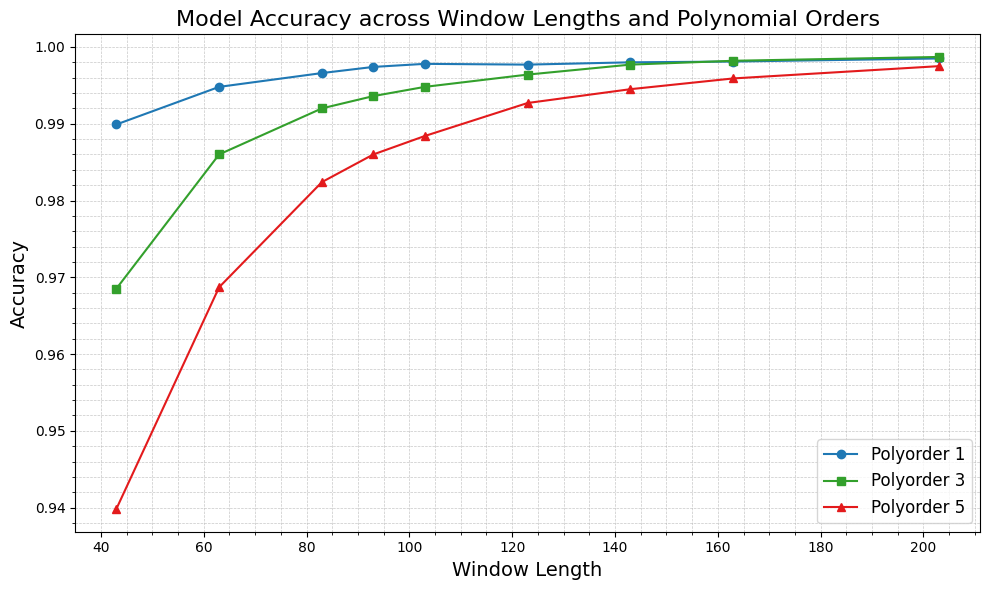
\includegraphics[width=6.0016in,height=3.5819in]{a0000-img008.png}}


\subsubsection[Figure: KNN model accuracy across different window lengths and polynomial
orders]{\textstyleInternetlink{\textbf{\textcolor[HTML]{1F3763}{Figure:}}\textcolor[HTML]{1F3763}{ KNN model accuracy
across different window lengths and polynomial orders}}}

\bigskip


\bigskip

\subsection{Signal Visualization}
Polyorder = 3, Window Size = 203


\bigskip

Alert Data


\lfbox[margin-bottom=0.0028in,margin-top=0mm,margin-right=0mm,margin-left=0mm,border-style=none,padding=0mm,vertical-align=top]{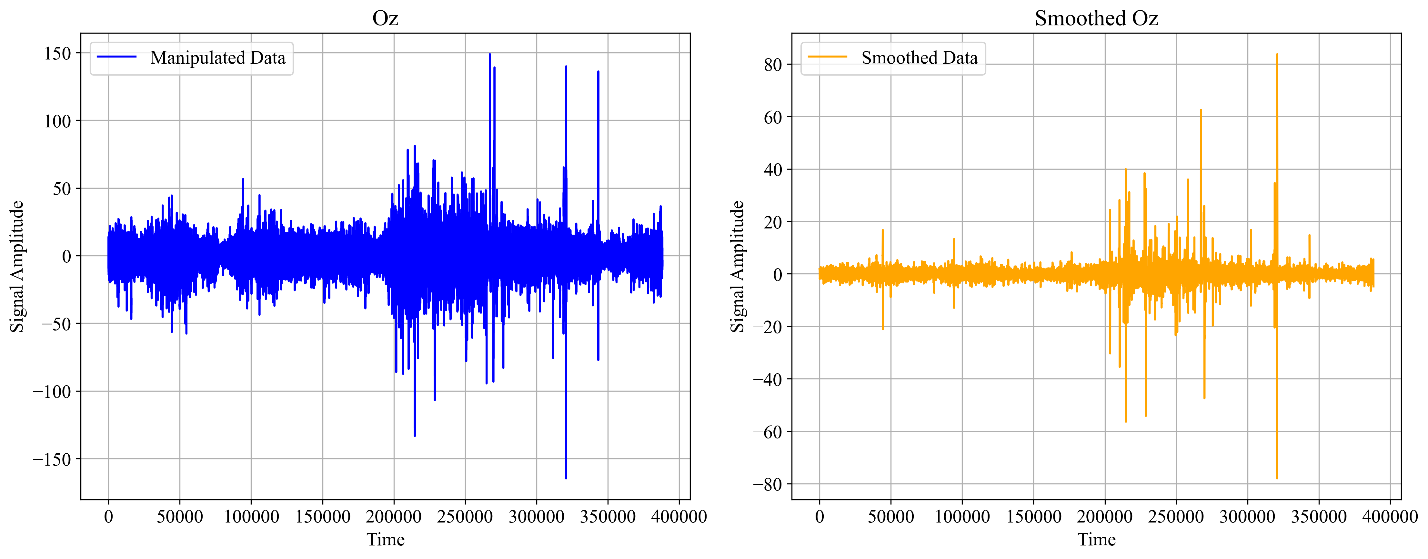
\includegraphics[width=6.489in,height=2.539in]{a0000-img009.png}}



\lfbox[margin=0mm,border-style=none,padding=0mm,vertical-align=top]{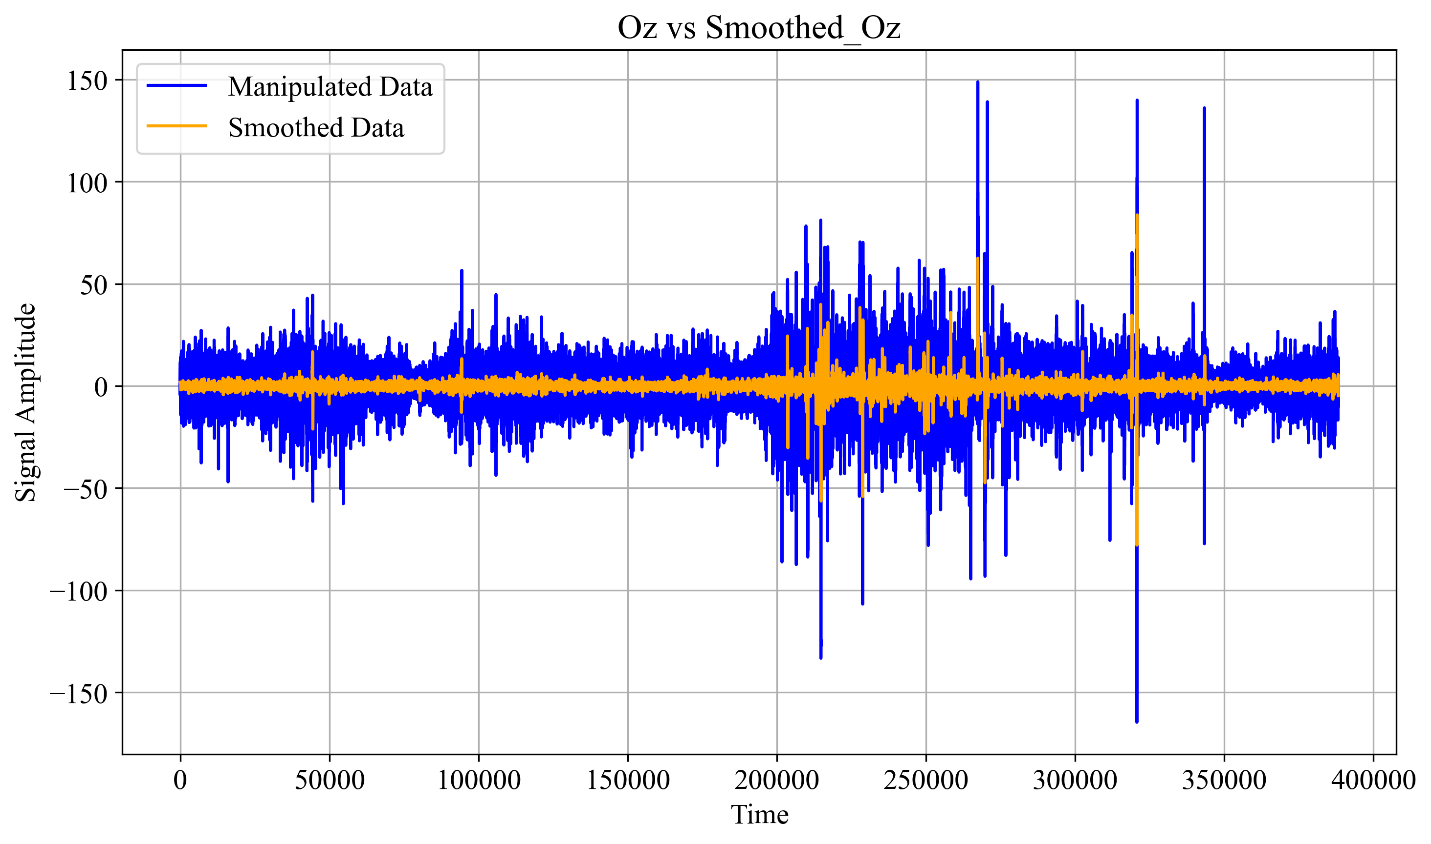
\includegraphics[width=6.5in,height=3.839in]{a0000-img010.png}}



\bigskip

\subsubsection[Figure: Alert Data Visualization of unfiltered EEG signals (Oz) vs. filtered Oz
signals.]{\textbf{Figure:} Alert Data Visualization of unfiltered EEG signals (Oz) vs. filtered Oz signals.}

\bigskip

Drowsy Data


\lfbox[margin-bottom=0.0028in,margin-top=0mm,margin-right=0mm,margin-left=0mm,border-style=none,padding=0mm,vertical-align=top]{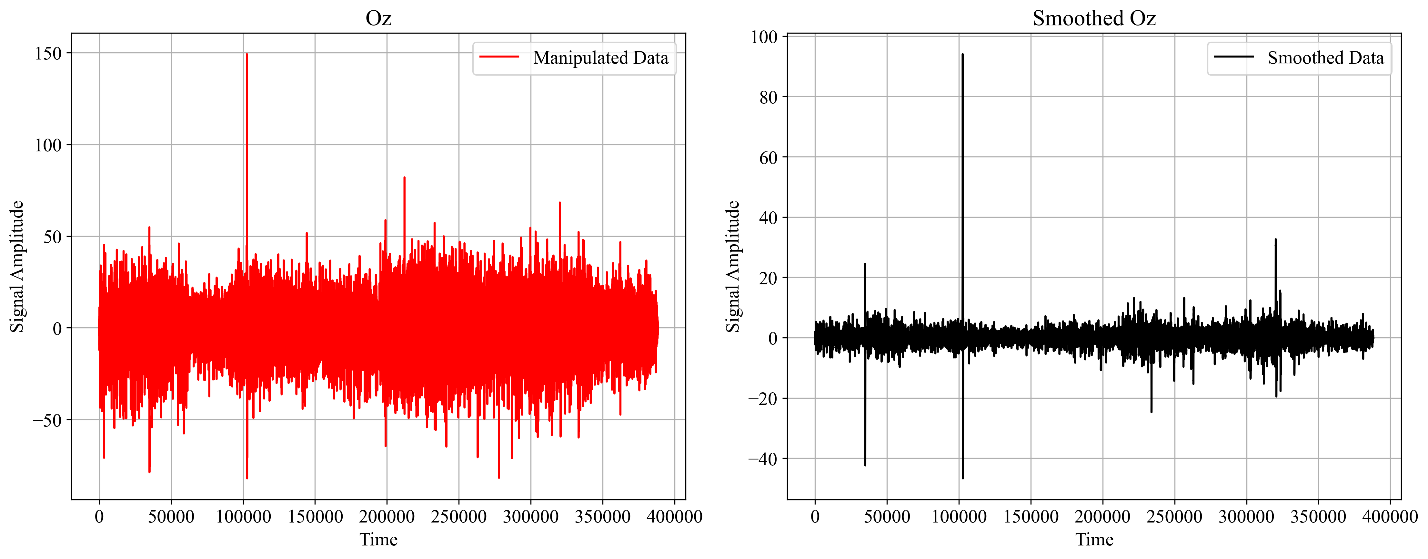
\includegraphics[width=6.489in,height=2.539in]{a0000-img011.png}}



\bigskip


\lfbox[margin=0mm,border-style=none,padding=0mm,vertical-align=top]{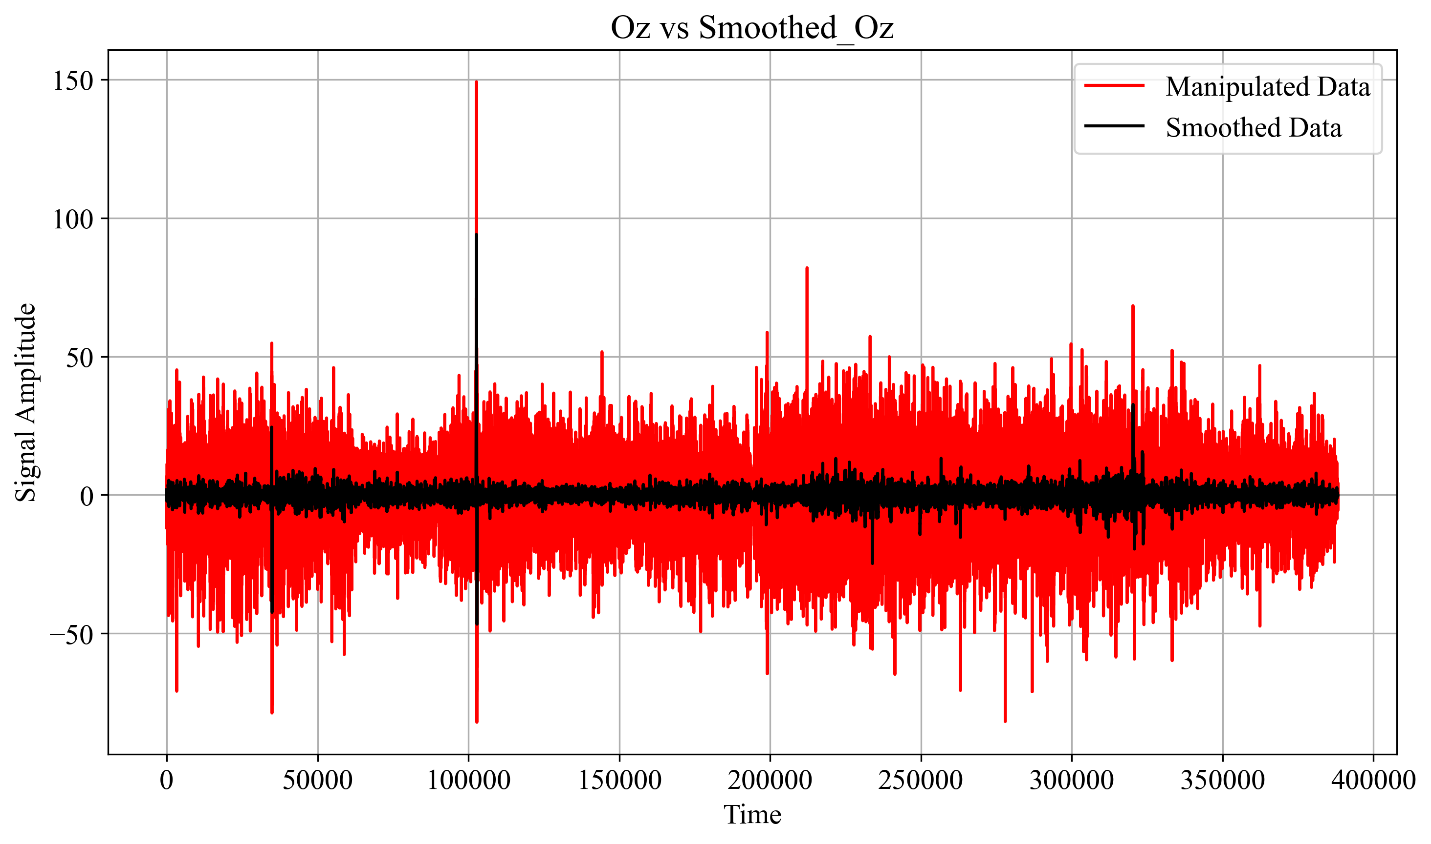
\includegraphics[width=6.5in,height=3.839in]{a0000-img012.png}}



\bigskip


\bigskip

\subsubsection[Figure: Drowsy Data visualization of unfiltered EEG signals (Oz) vs. filtered Oz
signals.]{\textbf{Figure:} Drowsy Data visualization of unfiltered EEG signals (Oz) vs. filtered Oz signals.}

\bigskip


\bigskip


\bigskip

{\centering
\textstyleHeadingiiChar{Machine Learning Evaluation with Savitzky-Golay Filter}\textbf{ }
\par}

{\centering
(Polyorder: 3, Window Size: 203)
\par}


\bigskip


\bigskip

\begin{flushleft}
\tablefirsthead{}
\tablehead{}
\tabletail{}
\tablelasttail{}
\begin{supertabular}{|m{1.1094599in}|m{0.70945984in}|m{0.68865985in}|m{0.6608598in}|m{0.6608598in}|m{0.8122598in}|m{1.2997599in}|}
\hline
{\bfseries Algorithm} &
\centering{\bfseries Accuracy} &
\centering{\bfseries Precision} &
\centering{\bfseries Recall} &
\centering{\bfseries F1-score} &
\centering{\bfseries AUC-ROC} &
\centering\arraybslash{\bfseries Training Times (s)}\\\hline
{\bfseries KNN} &
0.998693 &
0.999265 &
0.998119 &
0.998691 &
0.998693 &
0.07\\\hline
{\bfseries Random Forest} &
0.992491 &
0.996493 &
0.988456 &
0.992458 &
0.992490 &
617.77\\\hline
{\bfseries XGBoost} &
0.959991 &
0.971537 &
0.947716 &
0.959478 &
0.959986 &
6.72\\\hline
{\bfseries Decision Tree} &
0.924586 &
0.927525 &
0.921084 &
0.924293 &
0.924585 &
57.02\\\hline
{\bfseries Extra Trees} &
0.995943 &
0.998394 &
0.993481 &
0.995931 &
0.995942 &
154.29\\\hline
\end{supertabular}
\end{flushleft}

\bigskip

\subsubsection[Table: Machine Learning Evaluation with Filtered Dataset]{\textbf{Table:} Machine Learning Evaluation
with Filtered Dataset}
\centering
\lfbox[margin=0mm,border-style=none,padding=0mm,vertical-align=top]{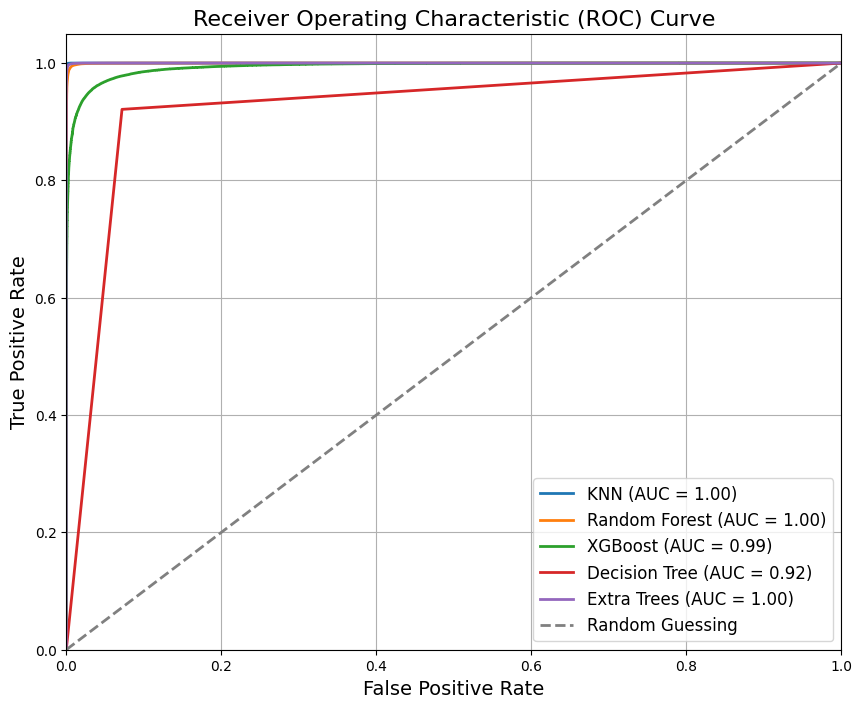
\includegraphics[width=4.5661in,height=3.7516in]{a0000-img013.png}}
\par

\bigskip

\subsubsection[Figure: ROC Curve for Machine Learning Results with Filtered Dataset.]{\textbf{Figure:} ROC Curve for
Machine Learning Results with Filtered Dataset.}

\bigskip


\bigskip


\bigskip


\bigskip


\bigskip


\bigskip

\section[Feature Selection {}- Shapley Approximation (shap)]{\textbf{Feature Selection - Shapley Approximation (shap)}}
The dataset is split into training and testing sets, with 80\% for training and 20\% for testing. XGBoost classifier is
trained on the training data. GPU acceleration is utilized for faster computation, and the number of trees is set to
5000. SHAP is employed for interpreting the XGBoost model predictions. SHAP values are calculated for the test dataset
to understand the contribution of each feature to the model's output. Feature importance is determined based on the
absolute mean SHAP values across all instances in the test dataset.

\textbf{Feature Importance Plot:} A horizontal bar plot is created to illustrate the importance of each feature, with
annotations showing the numerical values of importance.


\bigskip

\centering
\lfbox[margin=0mm,border-style=none,padding=0mm,vertical-align=top]{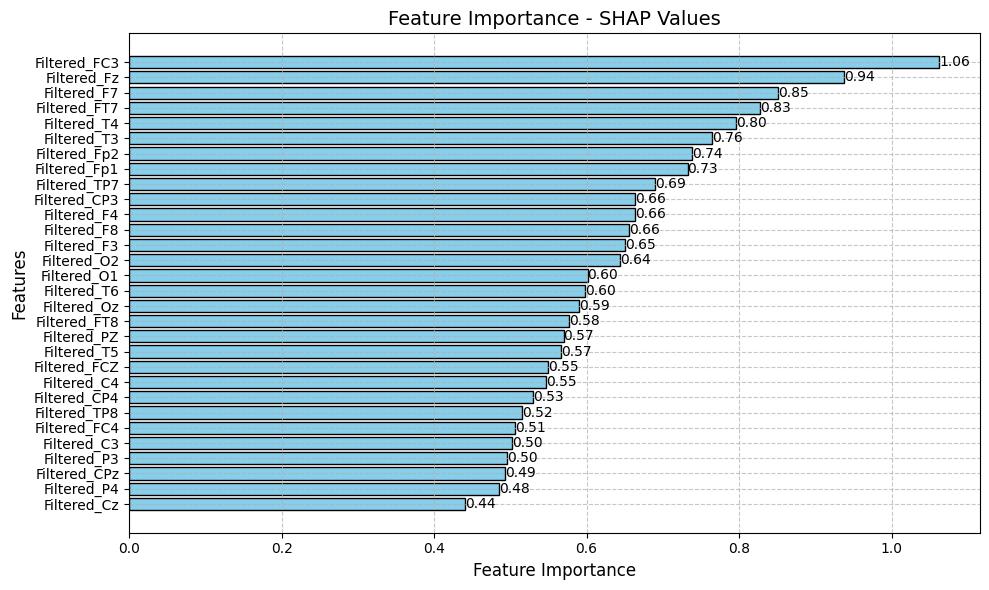
\includegraphics[width=6.5in,height=3.8799in]{a0000-img014.png}}
\par
\subsubsection[]{\rmfamily }
\subsubsection[Figure: Feature Importance SHAP Values]{\textbf{Figure:} Feature Importance SHAP Values}

\bigskip


\bigskip


\bigskip


\bigskip


\bigskip


\bigskip


\bigskip

\textbf{SHAP Summary Plot:} A summary plot is generated to visualize the distribution of SHAP values for each feature.


\bigskip


\bigskip

\centering
\lfbox[margin-bottom=0.0091in,margin-top=0mm,margin-right=0mm,margin-left=0mm,border-style=none,padding=0mm,vertical-align=top]{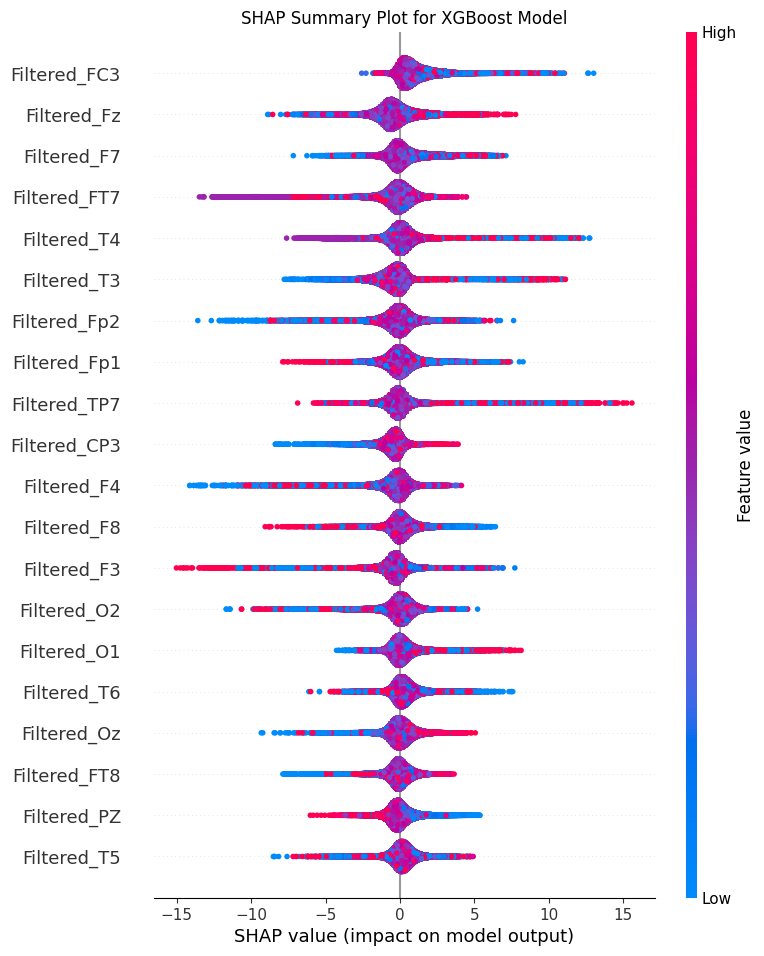
\includegraphics[width=5.1354in,height=6.4283in]{a0000-img015.png}}
\par

\bigskip

\subsubsection[Figure: Summary Plot for Feature Impact Distribution.]{\textbf{Figure:} Summary Plot for Feature Impact
Distribution.}

\bigskip


\bigskip

\centering
\lfbox[margin-bottom=0.0098in,margin-top=0mm,margin-right=0mm,margin-left=0mm,border-style=none,padding=0mm,vertical-align=top]{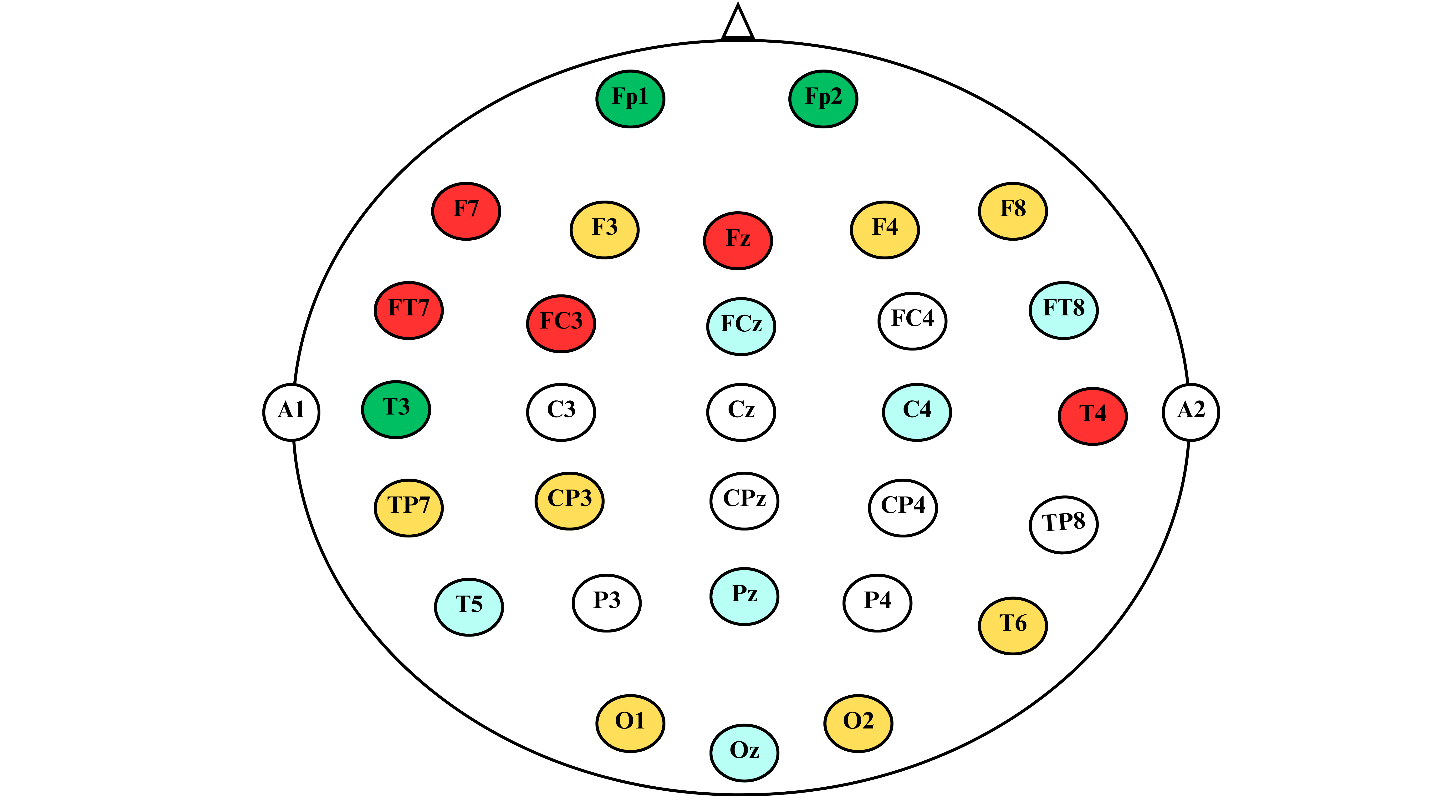
\includegraphics[width=3.9945in,height=3.1783in]{a0000-img016.png}}
\par

\bigskip

\subsubsection[Figure: Electrode Layout on EEG Cap Sorted by Feature Importance Values]{\textbf{Figure:} Electrode
Layout on EEG Cap Sorted by Feature Importance Values}

\bigskip

\textbf{Table of Feature Importance with Corresponding Denotations}

\begin{flushleft}
\tablefirsthead{}
\tablehead{}
\tabletail{}
\tablelasttail{}
\begin{supertabular}{|m{1.1254599in}|m{0.6504598in}|m{3.3934598in}|m{1.5518599in}|}
\hline
\centering{\bfseries Importance} &
\centering{\bfseries Total Features} &
\centering{\bfseries Features} &
\centering\arraybslash{\bfseries Denotations}\\\hline
\centering{\bfseries ${\geq}$ 0.80} &
\centering 5 &
FC3, Fz, F7, FT7, T4 &

\lfbox[margin-right=0.0063in,margin-top=0mm,margin-bottom=0mm,margin-left=0mm,border-style=none,padding=0mm,vertical-align=top]{
\includegraphics[width=0.328in,height=0.2937in]{a0000-img017.png}}
\\\hline
\centering{\bfseries ${\geq}$ 0.70} &
\centering 8 &
FC3, Fz, F7, FT7, T4, T3, Fp2, Fp1 &

\lfbox[margin-right=0.0043in,margin-top=0mm,margin-bottom=0mm,margin-left=0mm,border-style=none,padding=0mm,vertical-align=top]{
\includegraphics[width=0.6008in,height=0.2945in]{a0000-img017.png}}
\\\hline
\centering{\bfseries ${\geq}$ 0.60} &
\centering 16 &
FC3, Fz, F7, FT7, T4, T3, Fp2, Fp1, TP7, CP3, F4, F8, F3, O2, O1, T6 &

\lfbox[margin-bottom=0.0098in,margin-top=0mm,margin-right=0mm,margin-left=0mm,border-style=none,padding=0mm,vertical-align=top]{
\includegraphics[width=0.8846in,height=0.261in]{a0000-img017.png}}
\\\hline
\centering{\bfseries ${\geq}$ 0.55} &
\centering 22 &
FC3, Fz, F7, FT7, T4, T3, Fp2, Fp1, TP7, CP3, F4, F8, F3, O2, O1, T6, Oz, FT8, PZ, T5, FCZ, C4. &

\lfbox[margin-bottom=0.0071in,margin-top=0mm,margin-right=0mm,margin-left=0mm,border-style=none,padding=0mm,vertical-align=top]{
\includegraphics[width=1.1874in,height=0.2846in]{a0000-img018.png}}
\\\hline
\centering{\bfseries ${\geq}$ 0.40} &
\centering 30 &
FC3, Fz, F7, FT7, T4, T3, Fp2, Fp1, TP7, CP3, F4, F8, F3, O2, O1, T6, Oz, FT8, PZ, T5, FCZ, C4, CP4, TP8, FC4, C3, P3,
CPz, P4, Cz &

\lfbox[margin=0mm,border-style=none,padding=0mm,vertical-align=top]{
\includegraphics[width=1.4811in,height=0.2783in]{a0000-img017.png}}
\\\hline
\end{supertabular}
\end{flushleft}

\bigskip

\subsubsection[Table: Feature Importance with Corresponding Denotations]{\textbf{Table:} Feature Importance with
Corresponding Denotations}

\bigskip


\bigskip

\subsection{References}
\centering
\lfbox[margin-bottom=0.0063in,margin-top=0mm,margin-right=0mm,margin-left=0mm,border-style=none,padding=0mm,vertical-align=top]{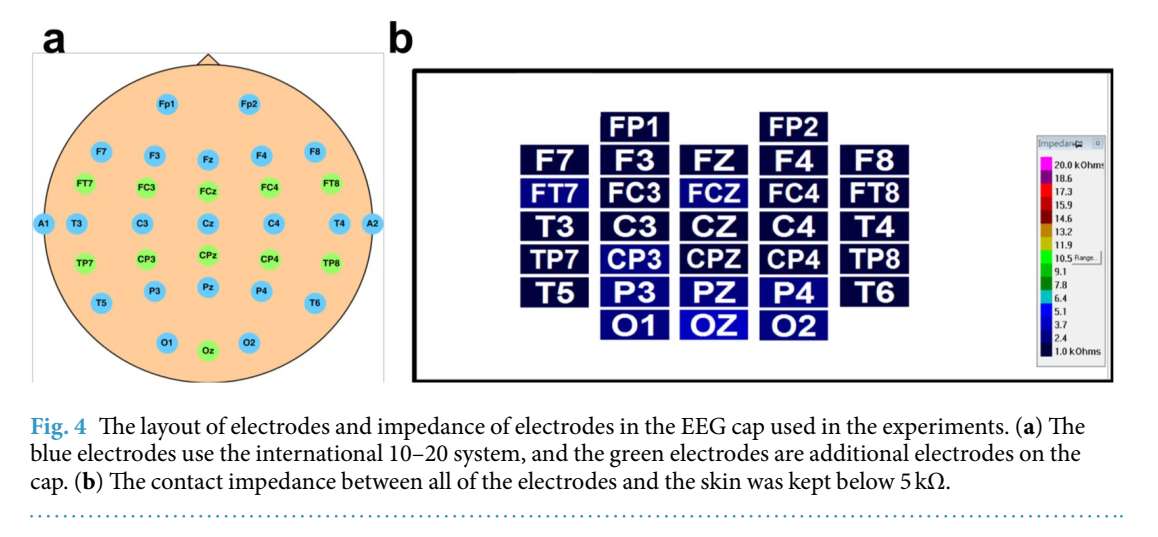
\includegraphics[width=6.5in,height=3.0146in]{a0000-img019.png}}
\par
{\centering
Image Source: \url{https://www.nature.com/articles/s41597-019-0027-4}
\par}


\bigskip


\bigskip


\bigskip


\bigskip


\bigskip


\bigskip


\bigskip


\bigskip


\bigskip


\bigskip


\bigskip


\bigskip


\bigskip


\bigskip


\bigskip


\bigskip


\bigskip


\bigskip


\bigskip


\bigskip


\bigskip


\bigskip


\bigskip


\bigskip


\bigskip


\bigskip


\bigskip


\bigskip


\bigskip


\bigskip


\bigskip

\section[Machine Learning Results]{\textbf{Machine Learning Results}}

\bigskip

\subsection{Mean Accuracy}
\begin{center}
\tablefirsthead{}
\tablehead{}
\tabletail{}
\tablelasttail{}
\begin{supertabular}{|m{1.5830599in}|m{0.41085985in}|m{1.0837599in}|m{0.66565984in}|m{0.9497598in}|m{0.8295598in}|}
\hline
{\bfseries Number of Features} &
{\bfseries KNN} &
{\bfseries Random Forest} &
{\bfseries XGBoost} &
{\bfseries Decision Tree} &
{\bfseries Extra Trees}\\\hline
5 Features &
0.84 &
0.83 &
0.72 &
0.74 &
0.83\\\hline
8 Features &
0.95 &
0.93 &
0.82 &
0.84 &
0.94\\\hline
16 Features &
0.99 &
0.98 &
0.92 &
0.90 &
0.99\\\hline
22 Features &
1.00 &
0.99 &
0.95 &
0.91 &
0.99\\\hline
30 Features &
1.00 &
0.99 &
0.96 &
0.91 &
0.99\\\hline
\end{supertabular}
\end{center}
\subsubsection[Table: Mean accuracy comparison across various feature sets.]{\textbf{Table:} Mean accuracy comparison
across various feature sets.}

\bigskip


\bigskip

\centering
\lfbox[margin=0mm,border-style=none,padding=0mm,vertical-align=top]{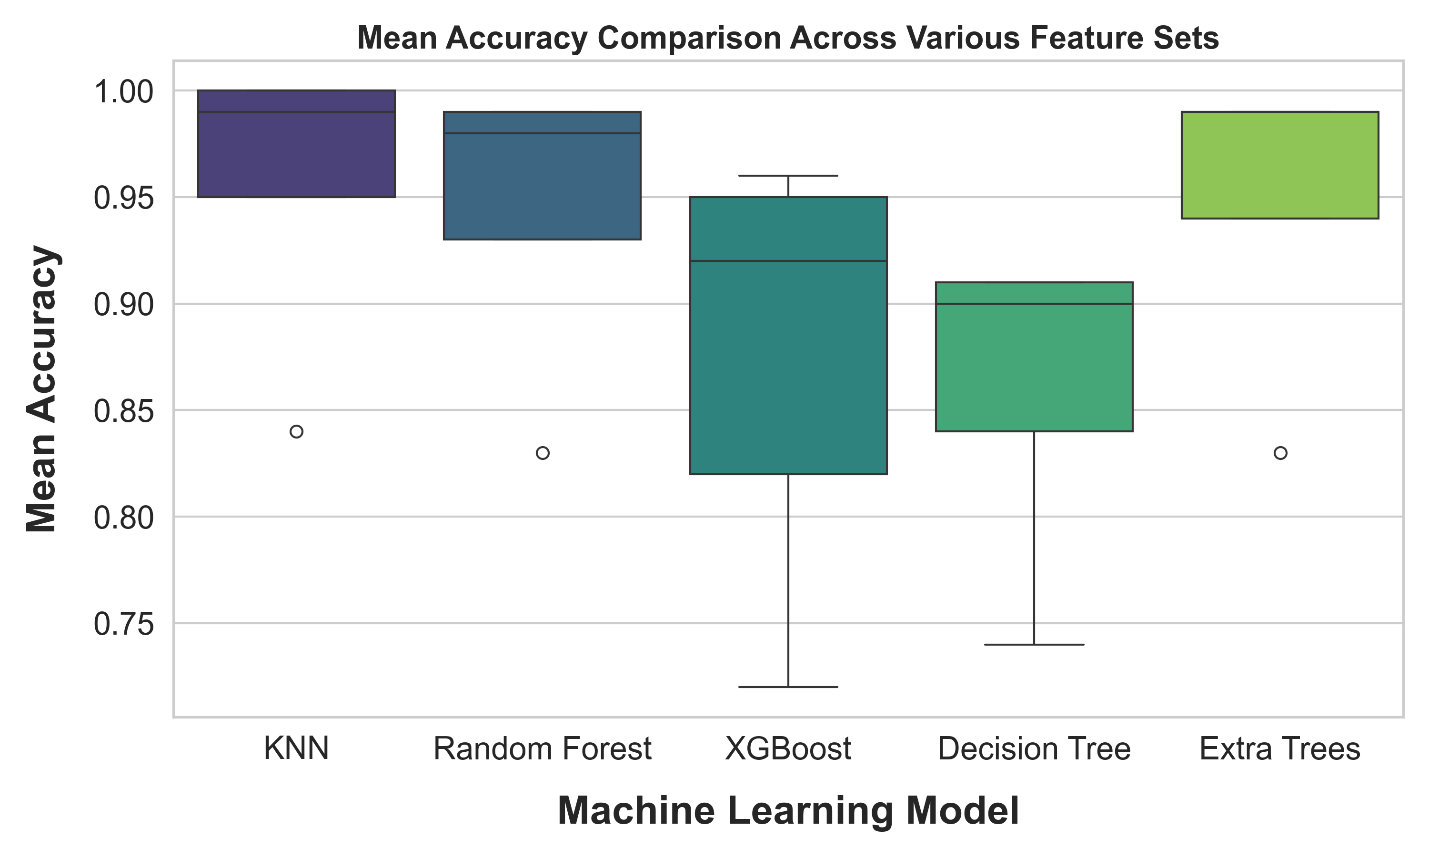
\includegraphics[width=6.5in,height=3.9in]{a0000-img020.png}}
\par
\subsubsection[Figure: Mean accuracy comparison across various feature sets.]{\textbf{Figure:} Mean accuracy comparison
across various feature sets.}

\bigskip


\bigskip


\bigskip


\bigskip


\bigskip

\subsection{Mean Precision}
\begin{center}
\tablefirsthead{}
\tablehead{}
\tabletail{}
\tablelasttail{}
\begin{supertabular}{|m{1.4900599in}|m{0.5393598in}|m{1.1087599in}|m{0.6719598in}|m{0.9837598in}|m{0.8580598in}|}
\hline
\centering{\bfseries Number of Features} &
\centering{\bfseries KNN} &
\centering{\bfseries Random Forest} &
\centering{\bfseries XGBoost} &
\centering{\bfseries Decision Tree} &
\centering\arraybslash{\bfseries Extra Trees}\\\hline
5 Features &
\centering 0.86 &
\centering 0.84 &
\centering 0.75 &
\centering 0.74 &
\centering\arraybslash 0.86\\\hline
8 Features &
\centering 0.96 &
\centering 0.95 &
\centering 0.84 &
\centering 0.84 &
\centering\arraybslash 0.96\\\hline
16 Features &
\centering 1.00 &
\centering 0.99 &
\centering 0.97 &
\centering 0.90 &
\centering\arraybslash 0.99\\\hline
22 Features &
\centering 1.00 &
\centering 0.99 &
\centering 0.96 &
\centering 0.91 &
\centering\arraybslash 1.00\\\hline
30 Features &
\centering 1.00 &
\centering 0.99 &
\centering 0.97 &
\centering 0.91 &
\centering\arraybslash 1.00\\\hline
\end{supertabular}
\end{center}
\subsubsection[Table: Mean precision comparison across various feature sets.]{\textbf{Table:} Mean precision comparison
across various feature sets.}

\bigskip

\centering
\lfbox[margin=0mm,border-style=none,padding=0mm,vertical-align=top]{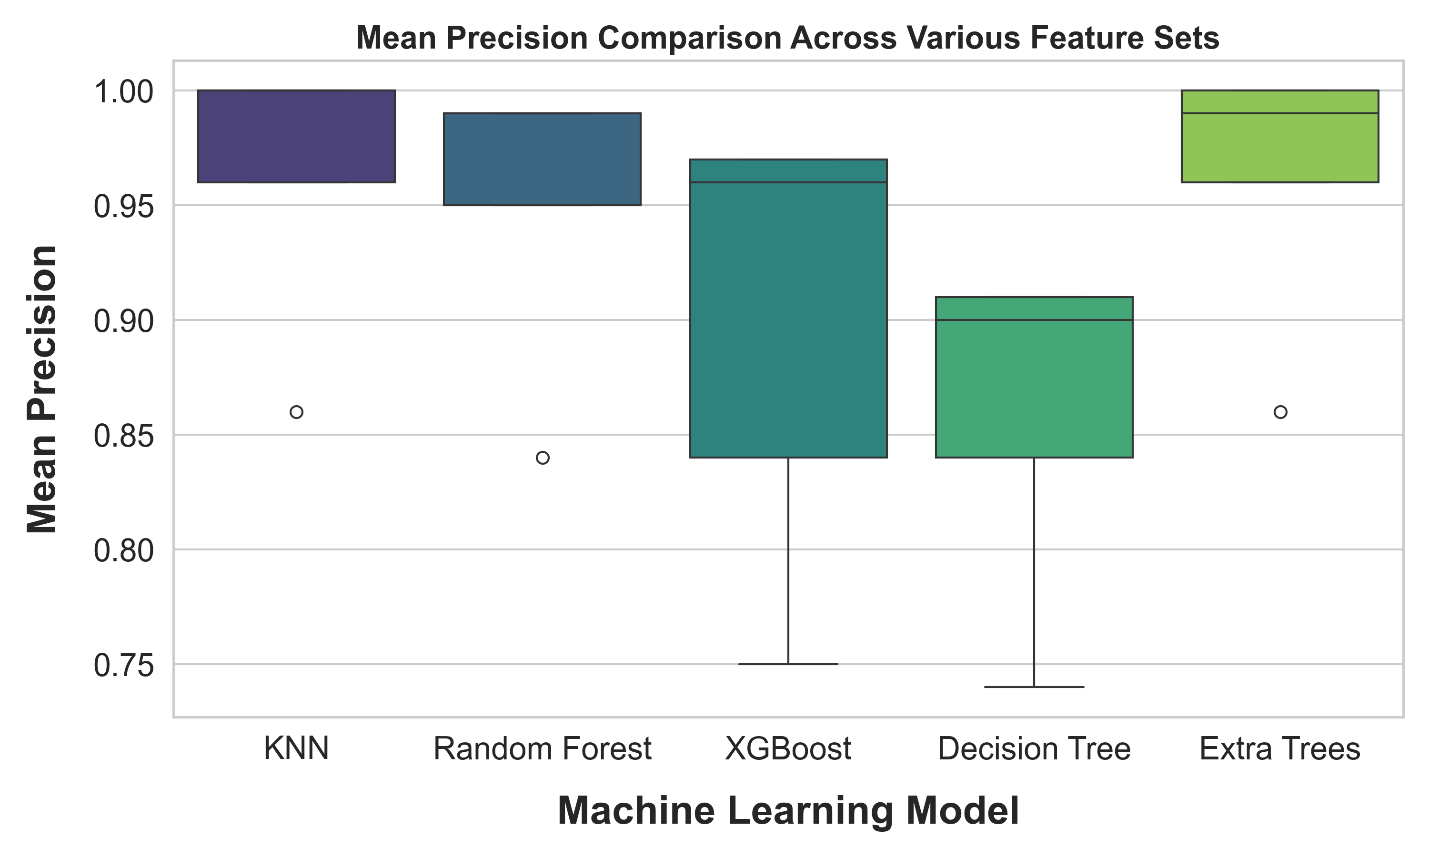
\includegraphics[width=6.5in,height=3.9in]{a0000-img021.png}}
\par
\subsubsection[Figure: Mean precision comparison across various feature sets.]{\textbf{Figure:} Mean precision
comparison across various feature sets.}

\bigskip


\bigskip


\bigskip


\bigskip


\bigskip


\bigskip

\subsection{Mean Recall}
\begin{center}
\tablefirsthead{}
\tablehead{}
\tabletail{}
\tablelasttail{}
\begin{supertabular}{|m{1.4212599in}|m{0.6011598in}|m{1.1087599in}|m{0.7337598in}|m{0.9837598in}|m{0.8587598in}|}
\hline
\centering{\bfseries Number of Features} &
\centering{\bfseries KNN} &
\centering{\bfseries Random Forest} &
\centering{\bfseries XGBoost} &
\centering{\bfseries Decision Tree} &
\centering\arraybslash{\bfseries Extra Trees}\\\hline
5 Features &
\centering 0.81 &
\centering 0.80 &
\centering 0.67 &
\centering 0.74 &
\centering\arraybslash 0.79\\\hline
8 Features &
\centering 0.94 &
\centering 0.91 &
\centering 0.79 &
\centering 0.83 &
\centering\arraybslash 0.91\\\hline
16 Features &
\centering 1.00 &
\centering 0.97 &
\centering 0.94 &
\centering 0.89 &
\centering\arraybslash 0.99\\\hline
22 Features &
\centering 0.99 &
\centering 0.98 &
\centering 0.93 &
\centering 0.90 &
\centering\arraybslash 0.99\\\hline
30 Features &
\centering 1.00 &
\centering 0.99 &
\centering 0.95 &
\centering 0.91 &
\centering\arraybslash 0.99\\\hline
\end{supertabular}
\end{center}
\subsubsection[Table: Mean recall comparison across various feature sets.]{\textbf{Table:} Mean recall comparison across
various feature sets.}
\centering
\lfbox[margin=0mm,border-style=none,padding=0mm,vertical-align=top]{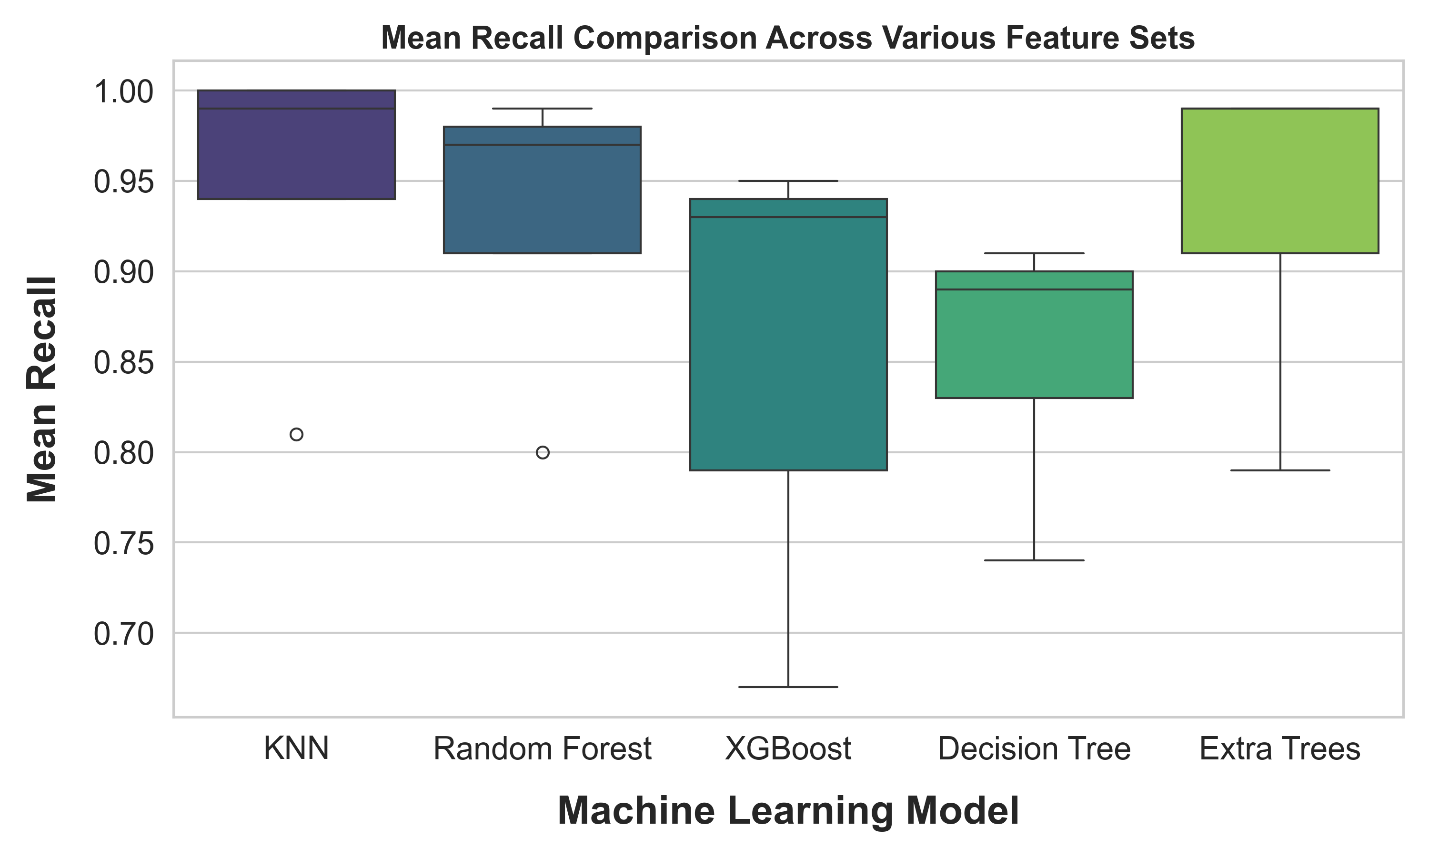
\includegraphics[width=6.5in,height=3.9in]{a0000-img022.png}}
\par
\subsubsection[Figure: Mean recall comparison across various feature sets.]{\textbf{Figure:} Mean recall comparison
across various feature sets.}

\bigskip


\bigskip


\bigskip


\bigskip


\bigskip


\bigskip


\bigskip

\subsection{Mean F1 Score}
\begin{center}
\tablefirsthead{}
\tablehead{}
\tabletail{}
\tablelasttail{}
\begin{supertabular}{|m{1.3809599in}|m{0.41085985in}|m{1.0830599in}|m{0.66565984in}|m{0.9497598in}|m{0.8309598in}|}
\hline
\centering{\bfseries Number of Features} &
\centering{\bfseries KNN} &
\centering{\bfseries Random Forest} &
\centering{\bfseries XGBoost} &
\centering{\bfseries Decision Tree} &
\centering\arraybslash{\bfseries Extra Trees}\\\hline
5 Features &
\centering 0.84 &
\centering 0.83 &
\centering 0.72 &
\centering 0.74 &
\centering\arraybslash 0.83\\\hline
8 Features &
\centering 0.95 &
\centering 0.93 &
\centering 0.81 &
\centering 0.84 &
\centering\arraybslash 0.93\\\hline
16 Features &
\centering 0.99 &
\centering 0.98 &
\centering 0.92 &
\centering 0.90 &
\centering\arraybslash 0.99\\\hline
22 Features &
\centering 1.00 &
\centering 0.99 &
\centering 0.94 &
\centering 0.91 &
\centering\arraybslash 0.99\\\hline
30 Features &
\centering 1.00 &
\centering 0.99 &
\centering 0.96 &
\centering 0.91 &
\centering\arraybslash 0.99\\\hline
\end{supertabular}
\end{center}

\bigskip

\subsubsection[Table: Mean F1 Score comparison across various feature sets.]{\textbf{Table:} Mean F1 Score comparison
across various feature sets.}

\bigskip

\centering
\lfbox[margin=0mm,border-style=none,padding=0mm,vertical-align=top]{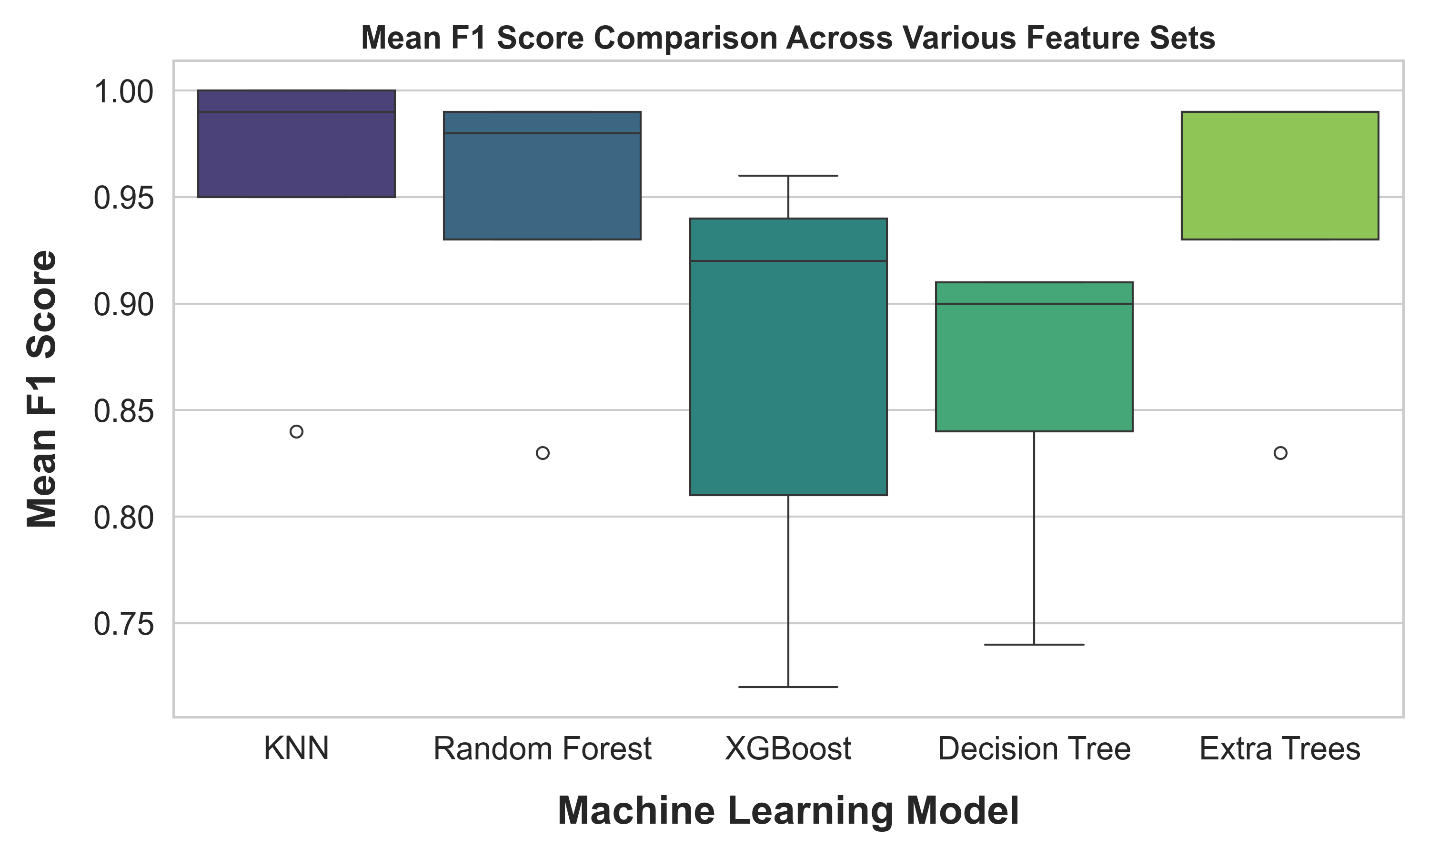
\includegraphics[width=6.5in,height=3.9in]{a0000-img023.png}}
\par

\bigskip


\bigskip

\subsubsection[Figure: Mean F1 Score comparison across various feature sets.]{\textbf{Figure:} Mean F1 Score comparison
across various feature sets.}

\bigskip


\bigskip


\bigskip


\bigskip


\bigskip

\subsection{Training Time of Machine Learning Model}
\begin{flushleft}
\tablefirsthead{}
\tablehead{}
\tabletail{}
\tablelasttail{}
\begin{supertabular}{|m{1.4490598in}|m{0.8302598in}|m{1.1511599in}|m{0.9906598in}|m{0.9900598in}|m{0.9906598in}|}
\hline
\centering{\bfseries Number of Features} &
\centering{\bfseries KNN} &
\centering{\bfseries Random Forest} &
\centering{\bfseries XGBoost} &
\centering{\bfseries Decision Tree} &
\centering\arraybslash{\bfseries Extra Trees}\\\hline
5 Features &
\centering 0.79 &
\centering 189.50 &
\centering 3.36 &
\centering 6.71 &
\centering\arraybslash 63.40\\\hline
8 Features &
\centering 1.11 &
\centering 196.92 &
\centering 4.02 &
\centering 11.41 &
\centering\arraybslash 69.11\\\hline
16 Features &
\centering 0.04 &
\centering 380.56 &
\centering 4.59 &
\centering 23.29 &
\centering\arraybslash 102.52\\\hline
22 Features &
\centering 0.05 &
\centering 380.34 &
\centering 5.22 &
\centering 31.97 &
\centering\arraybslash 110.24\\\hline
30 Features &
\centering 0.05 &
\centering 478.50 &
\centering 6.10 &
\centering 44.69 &
\centering\arraybslash 128.68\\\hline
\end{supertabular}
\end{flushleft}

\bigskip

\subsubsection[Table: Machine learning model training time across various feature sets]{\textbf{Table:} Machine learning
model training time across various feature sets}

\bigskip

\centering
\lfbox[margin=0mm,border-style=none,padding=0mm,vertical-align=top]{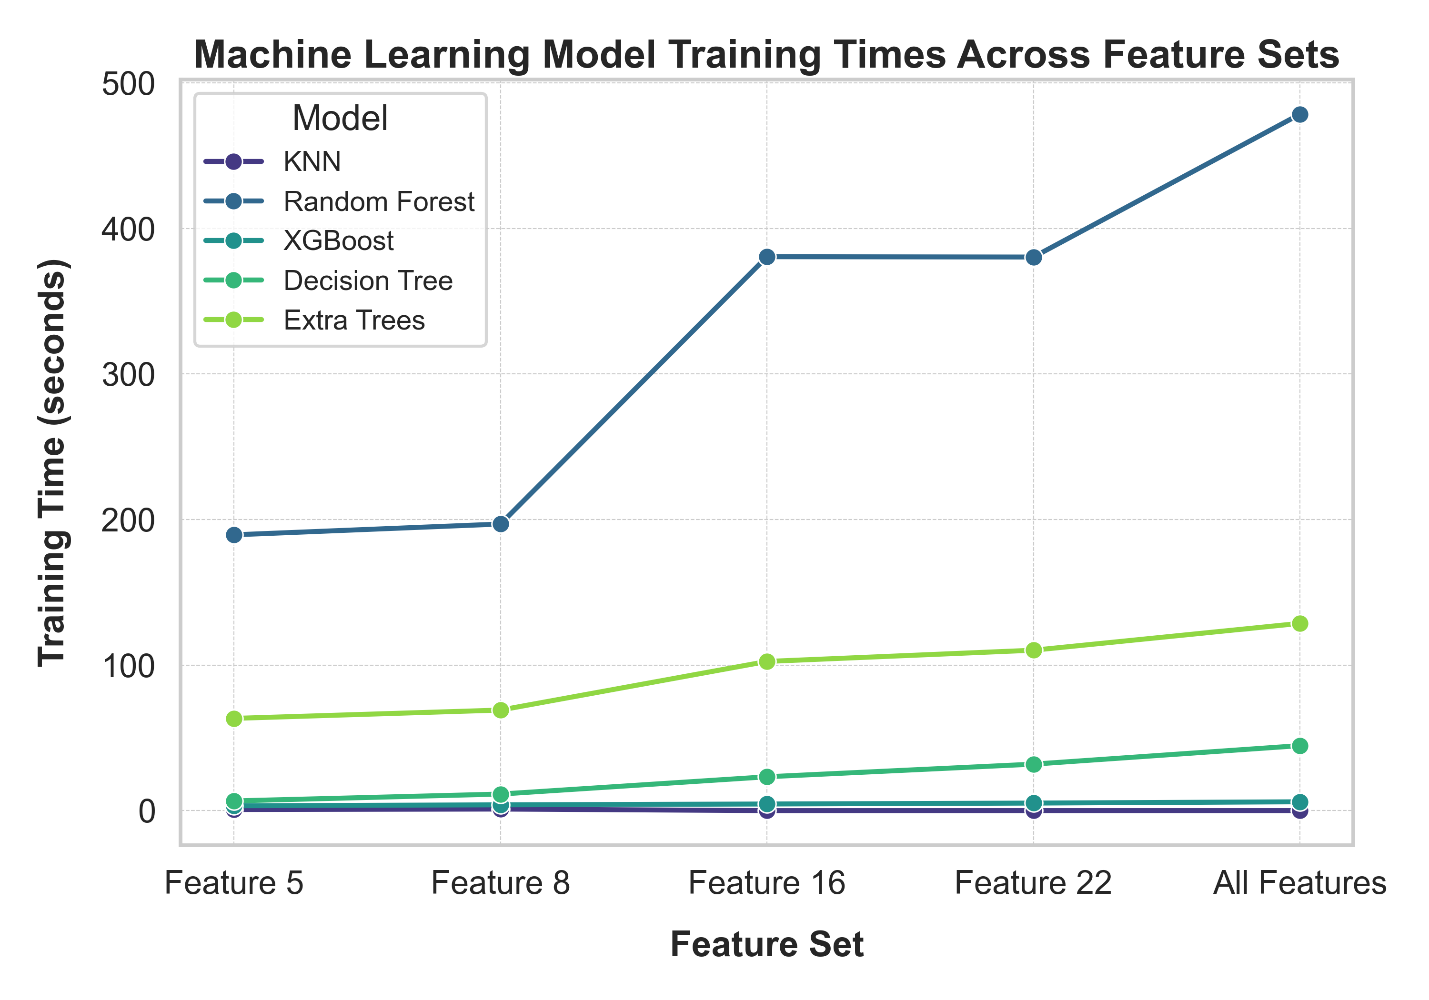
\includegraphics[width=6.5in,height=4.55in]{a0000-img024.png}}
\par

\bigskip

\subsubsection[Figure: Machine learning model training time across various feature sets]{\textbf{Figure:} Machine
learning model training time across various feature sets}

\bigskip

\subsection{Cross Validation}
\centering
\lfbox[margin-bottom=0.0071in,margin-top=0mm,margin-right=0mm,margin-left=0mm,border-style=none,padding=0mm,vertical-align=top]{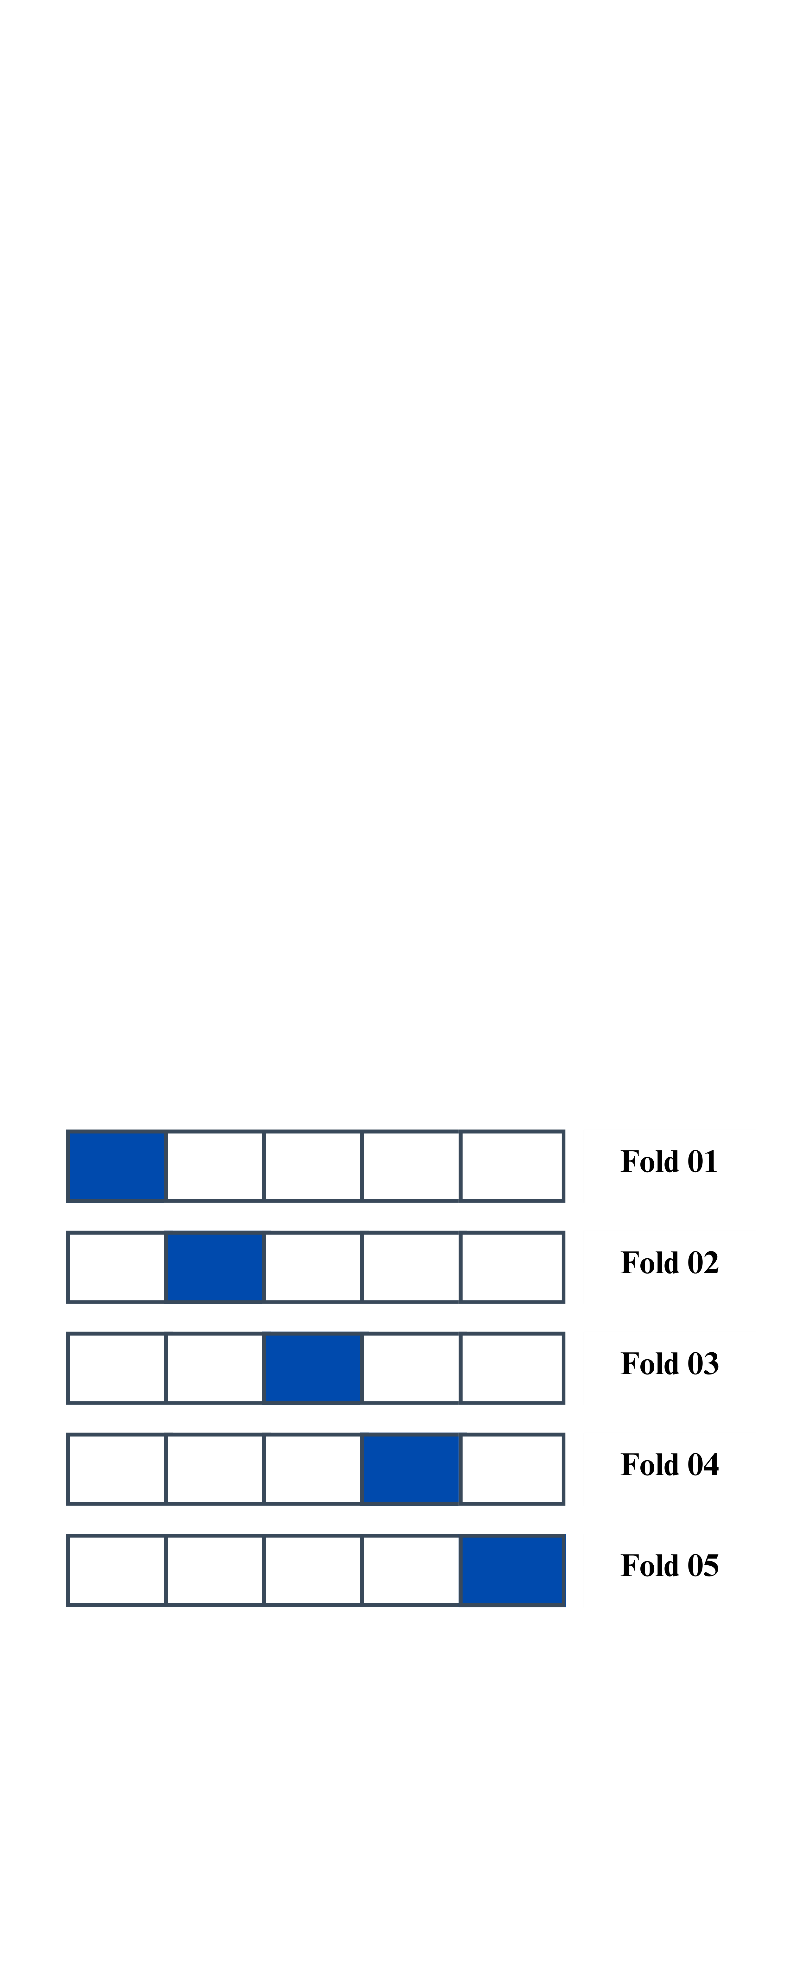
\includegraphics[width=3.361in,height=2.3681in]{a0000-img025.png}}

\lfbox[margin=0mm,border-style=none,padding=0mm,vertical-align=top]{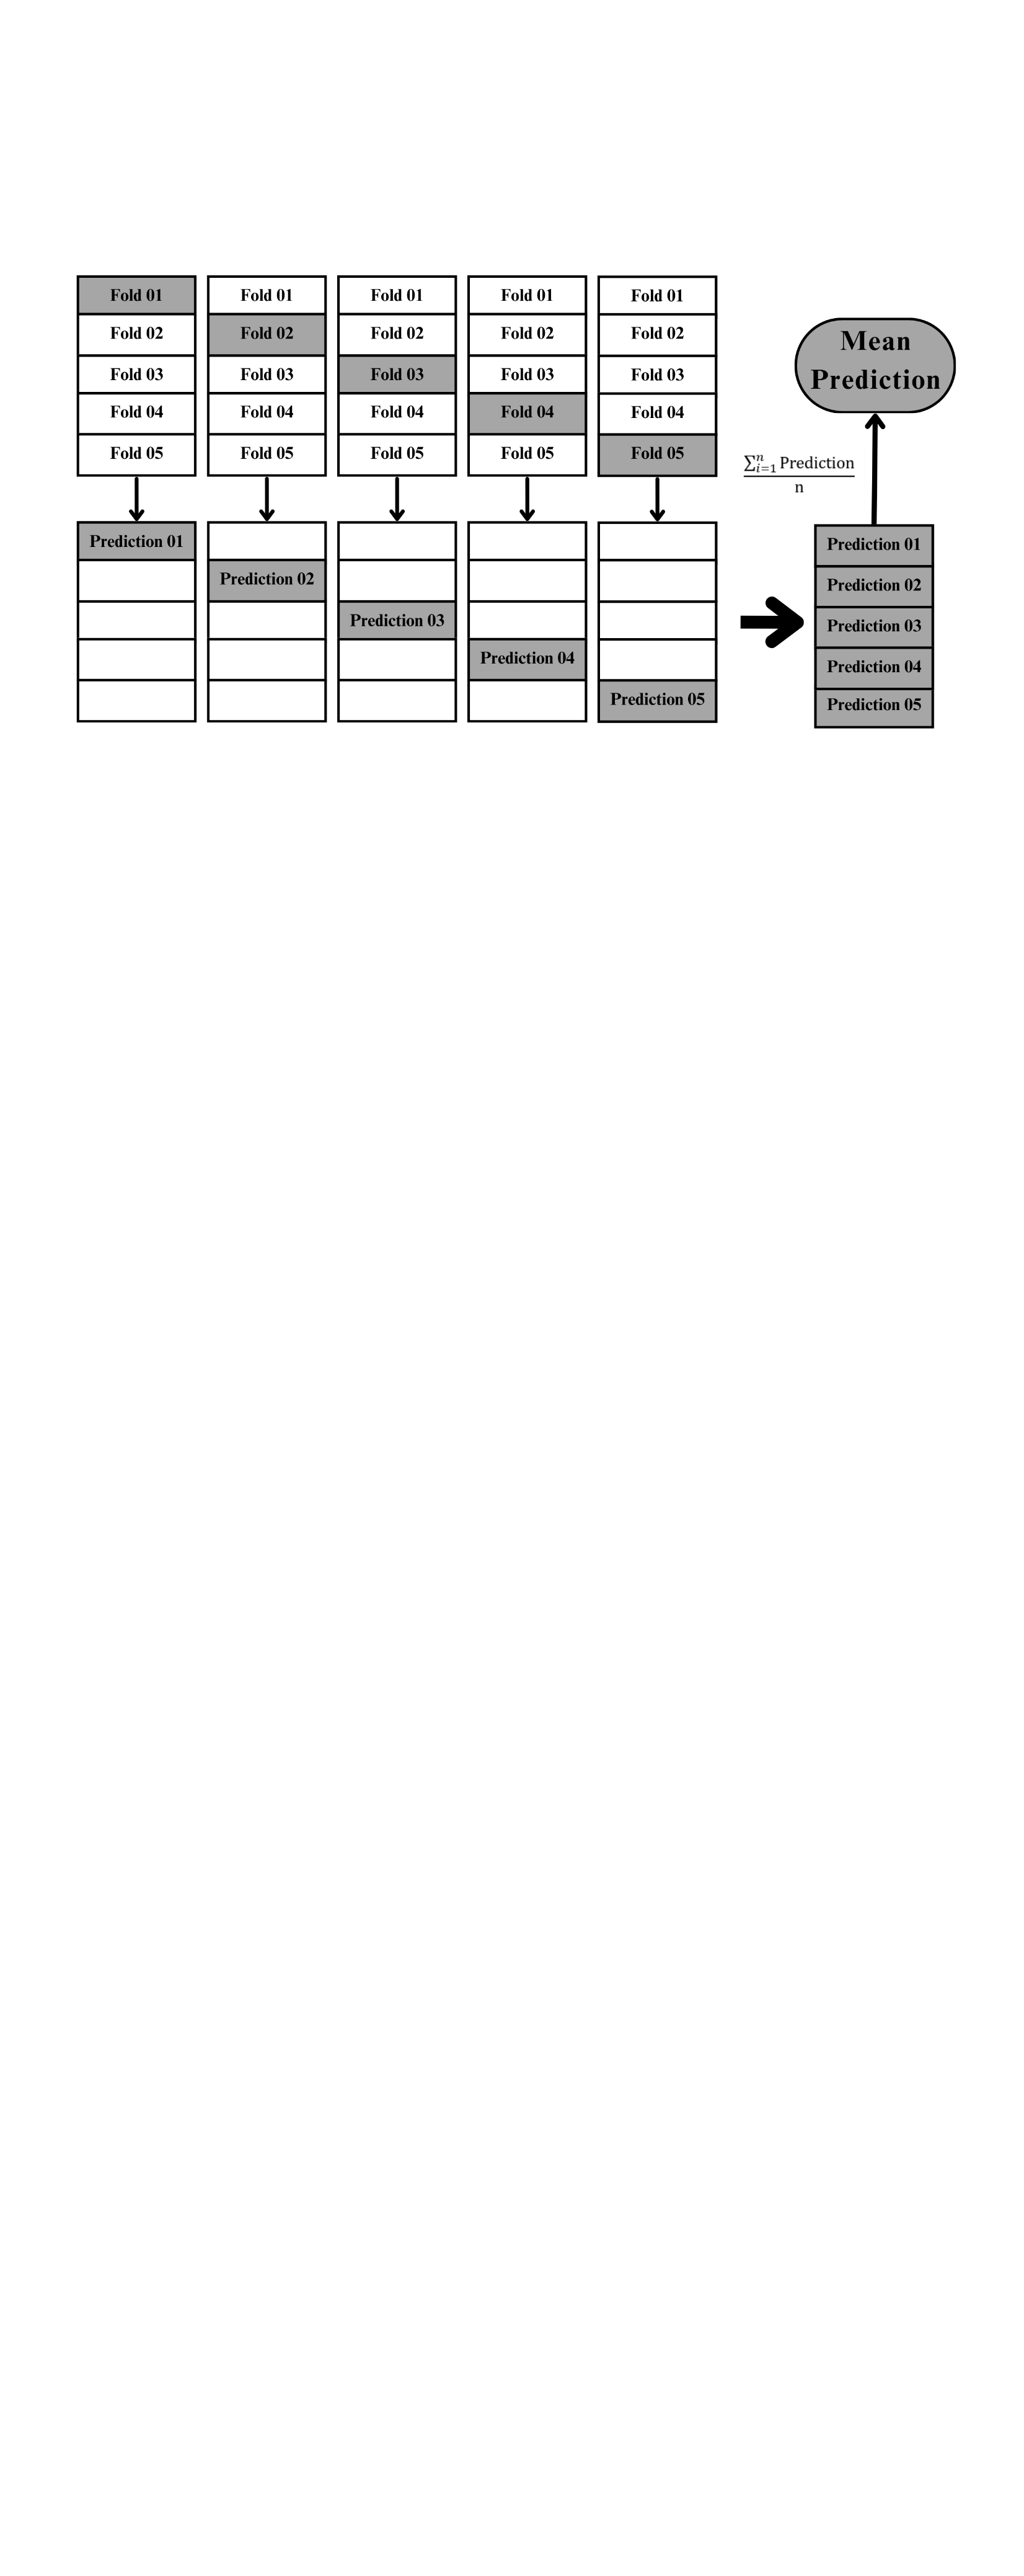
\includegraphics[width=6.798in,height=3.6528in]{a0000-img026.png}}
\par
\subsubsection[Figure: Cross Validation Workflow]{\textbf{Figure:} Cross Validation Workflow}

\bigskip


\bigskip


\bigskip


\bigskip


\bigskip


\bigskip


\bigskip


\bigskip

\section[Overall Performance Comparison]{\textbf{Overall Performance Comparison}}

\bigskip

\subsection{Mean Accuracy}
\begin{flushleft}
\tablefirsthead{}
\tablehead{}
\tabletail{}
\tablelasttail{}
\begin{supertabular}{|m{1.0268599in}|m{1.0268599in}|m{1.0275599in}|m{1.0268599in}|m{1.0275599in}|m{1.0268599in}|}
\hline
\centering{\bfseries Feature} &
\centering{\bfseries XGBoost} &
\centering{\bfseries Decision Tree} &
\centering{\bfseries Random Forest} &
\centering{\bfseries Extra Trees} &
\centering\arraybslash{\bfseries KNN}\\\hline
Feature 5 &
0.72 &
0.74 &
0.83 &
0.83 &
0.84\\\hline
Feature 8 &
0.82 &
0.84 &
0.93 &
0.94 &
0.95\\\hline
Feature 16 &
0.92 &
0.90 &
0.98 &
0.99 &
0.99\\\hline
Feature 22 &
0.95 &
0.91 &
0.99 &
0.99 &
1.00\\\hline
All Features &
0.96 &
0.91 &
0.99 &
0.99 &
1.00\\\hline
\end{supertabular}
\end{flushleft}

\bigskip

\centering
\lfbox[margin-right=0.0071in,margin-bottom=0.0071in,margin-top=0mm,margin-left=0mm,border-style=none,padding=0mm,vertical-align=top]{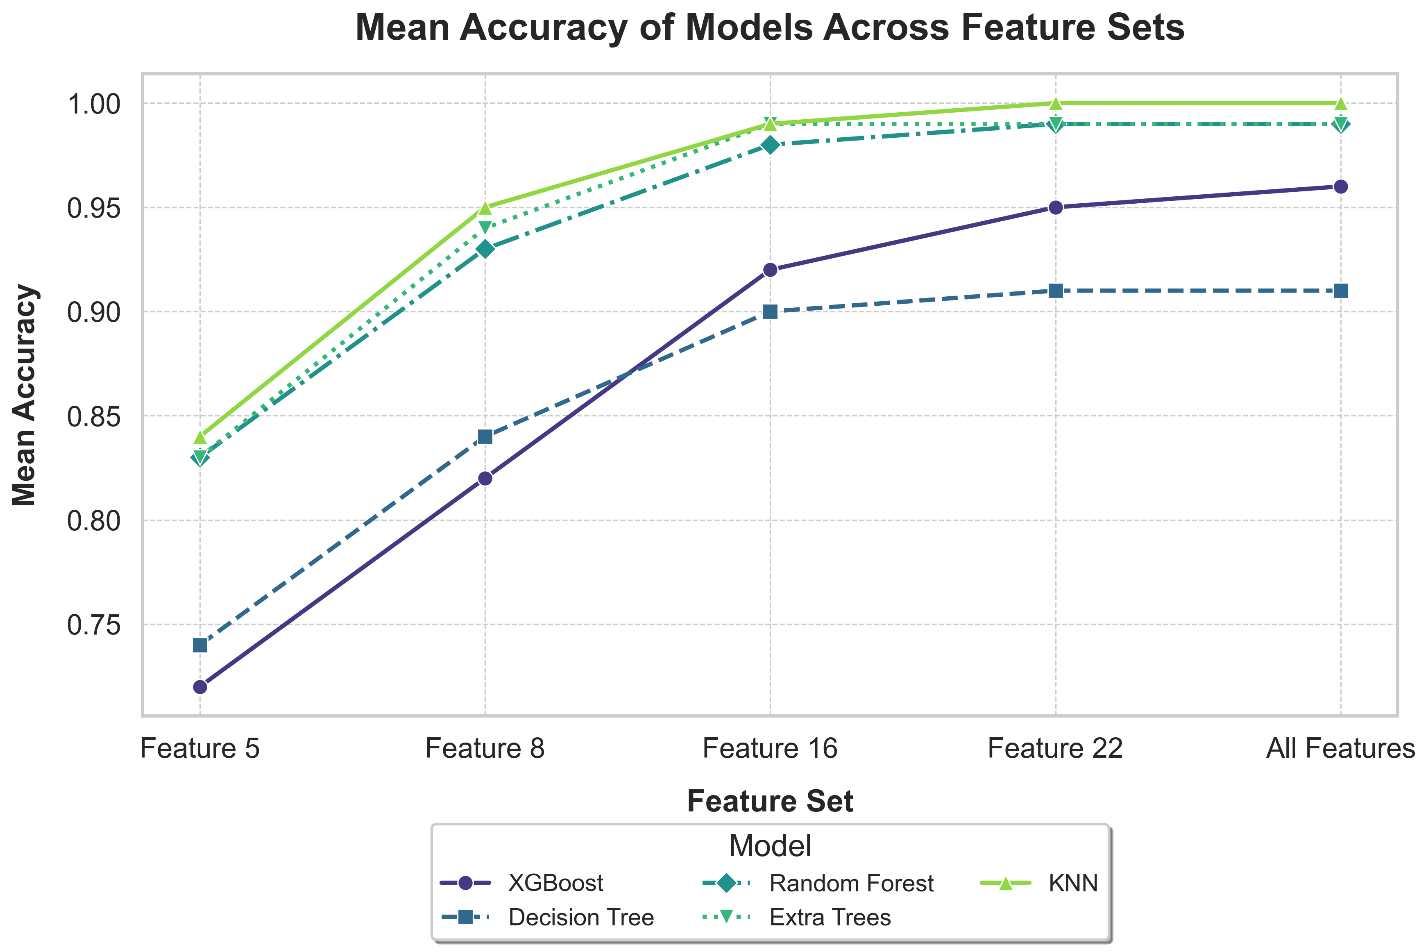
\includegraphics[width=6.4929in,height=4.3264in]{a0000-img027.png}}
\par

\bigskip

\subsubsection[Figure: Mean Accuracy Comparison of Machine Learning Models Across Feature Sets]{\textbf{Figure:} Mean
Accuracy Comparison of Machine Learning Models Across Feature Sets}

\bigskip


\bigskip

\subsection[Mean F1{}-Score]{Mean F1-Score}
\begin{flushleft}
\tablefirsthead{}
\tablehead{}
\tabletail{}
\tablelasttail{}
\begin{supertabular}{|m{1.0705599in}|m{1.0719599in}|m{1.0726599in}|m{1.0733598in}|m{1.0726599in}|m{1.0719599in}|}
\hline
\centering{\bfseries Feature} &
\centering{\bfseries XGBoost} &
\centering{\bfseries Decision Tree} &
\centering{\bfseries Random Forest} &
\centering{\bfseries Extra Trees} &
\centering\arraybslash{\bfseries KNN}\\\hline
{\bfseries Feature 5} &
0.72 &
0.74 &
0.83 &
0.83 &
0.84\\\hline
{\bfseries Feature 8} &
0.81 &
0.84 &
0.93 &
0.93 &
0.95\\\hline
{\bfseries Feature 16} &
0.92 &
0.90 &
0.98 &
0.99 &
0.99\\\hline
{\bfseries Feature 22} &
0.94 &
0.91 &
0.99 &
0.99 &
1.00\\\hline
{\bfseries All Features} &
0.96 &
0.91 &
0.99 &
0.99 &
1.00\\\hline
\end{supertabular}
\end{flushleft}

\bigskip

\centering
\lfbox[margin-right=0.0071in,margin-bottom=0.0071in,margin-top=0mm,margin-left=0mm,border-style=none,padding=0mm,vertical-align=top]{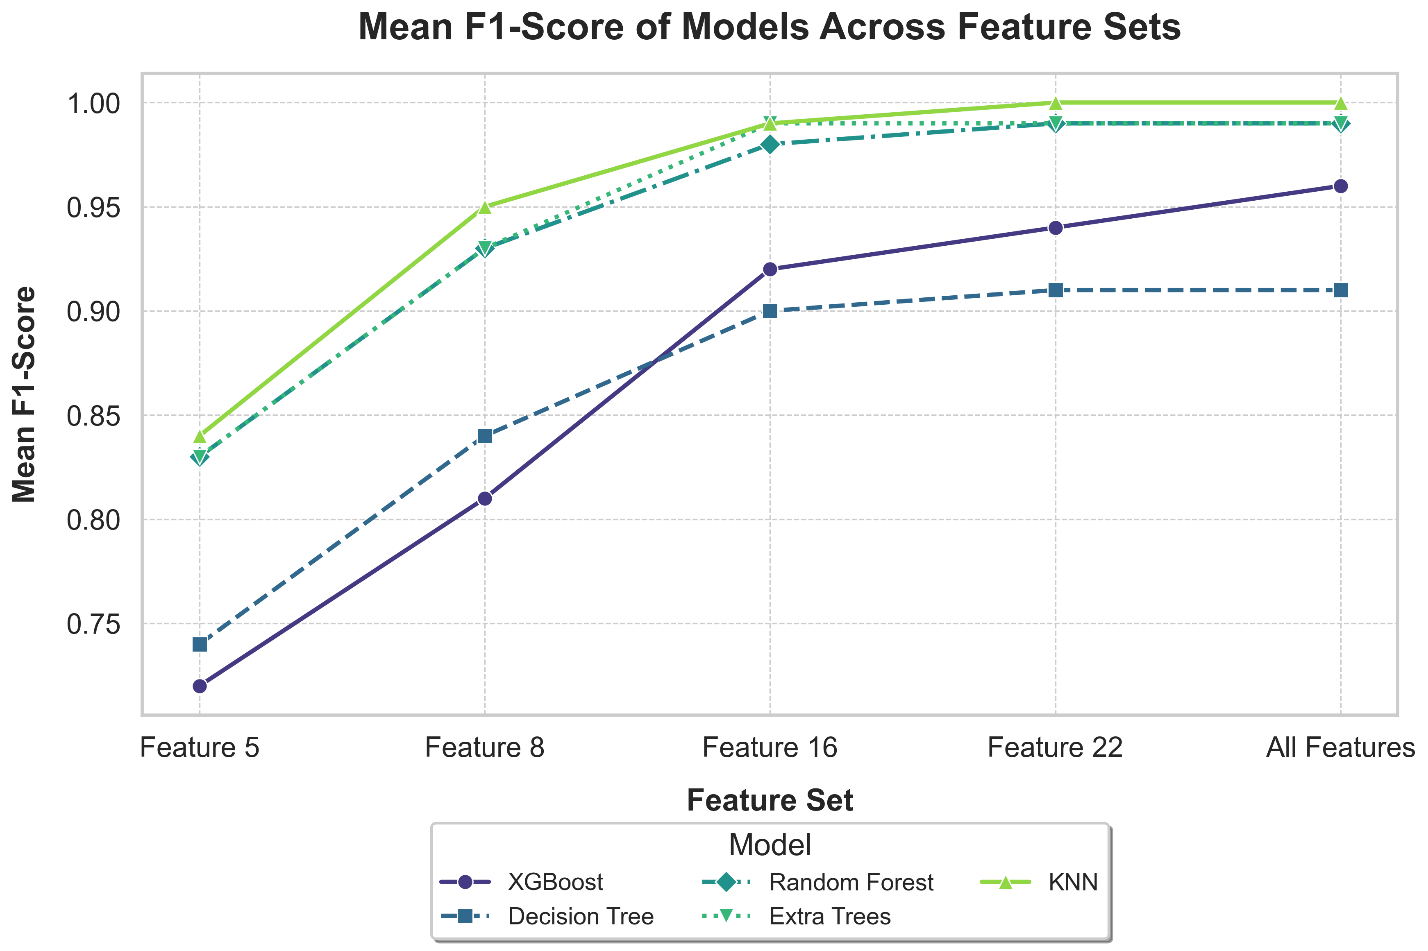
\includegraphics[width=6.4929in,height=4.3264in]{a0000-img028.png}}
\par

\bigskip

\subsubsection[Figure: Mean F1{}-Score Comparison of Machine Learning Models Across Feature Sets]{\textbf{Figure: }Mean
F1-Score Comparison of Machine Learning Models Across Feature Sets}

\bigskip


\bigskip


\bigskip

\subsection{Performance Comparison Using 16 Features}
\begin{flushleft}
\tablefirsthead{}
\tablehead{}
\tabletail{}
\tablelasttail{}
\begin{supertabular}{|m{2.24416in}|m{2.24486in}|m{2.24486in}|}
\hline
\centering{\bfseries Model} &
\centering{\bfseries Accuracy} &
\centering\arraybslash{\bfseries F1 Score}\\\hline
XGBoost &
\centering 0.92 &
\centering\arraybslash 0.92\\\hline
Decision Tree &
\centering 0.90 &
\centering\arraybslash 0.90\\\hline
Random Forest &
\centering 0.98 &
\centering\arraybslash 0.98\\\hline
Extra Trees &
\centering 0.99 &
\centering\arraybslash 0.99\\\hline
KNN &
\centering 0.99 &
\centering\arraybslash 0.99\\\hline
\end{supertabular}
\end{flushleft}

\bigskip


\bigskip


\bigskip

\centering
\lfbox[margin-right=0.0071in,margin-bottom=0.0071in,margin-top=0mm,margin-left=0mm,border-style=none,padding=0mm,vertical-align=top]{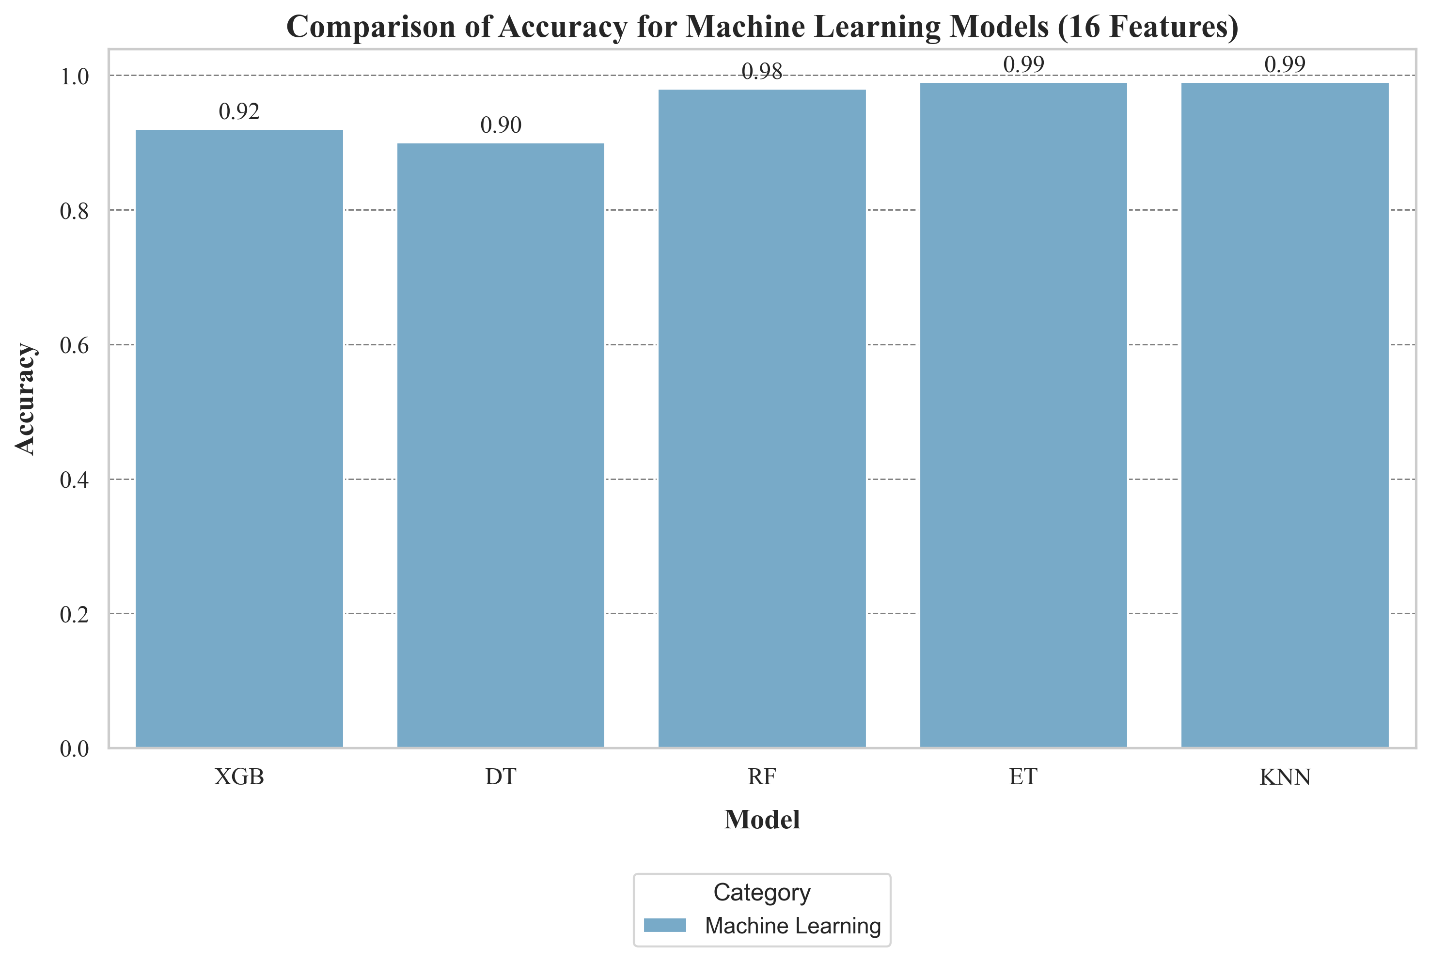
\includegraphics[width=6.4929in,height=4.3681in]{a0000-img029.png}}
\par
\subsubsection[\ \ Figure: Comparison of Accuracy Across Machine Learning Models Using 16 Features]{\ \ \textbf{Figure:}
Comparison of Accuracy Across Machine Learning Models Using 16 Features}

\bigskip


\bigskip


\bigskip


\bigskip

\centering
\lfbox[margin-right=0.0071in,margin-bottom=0.0071in,margin-top=0mm,margin-left=0mm,border-style=none,padding=0mm,vertical-align=top]{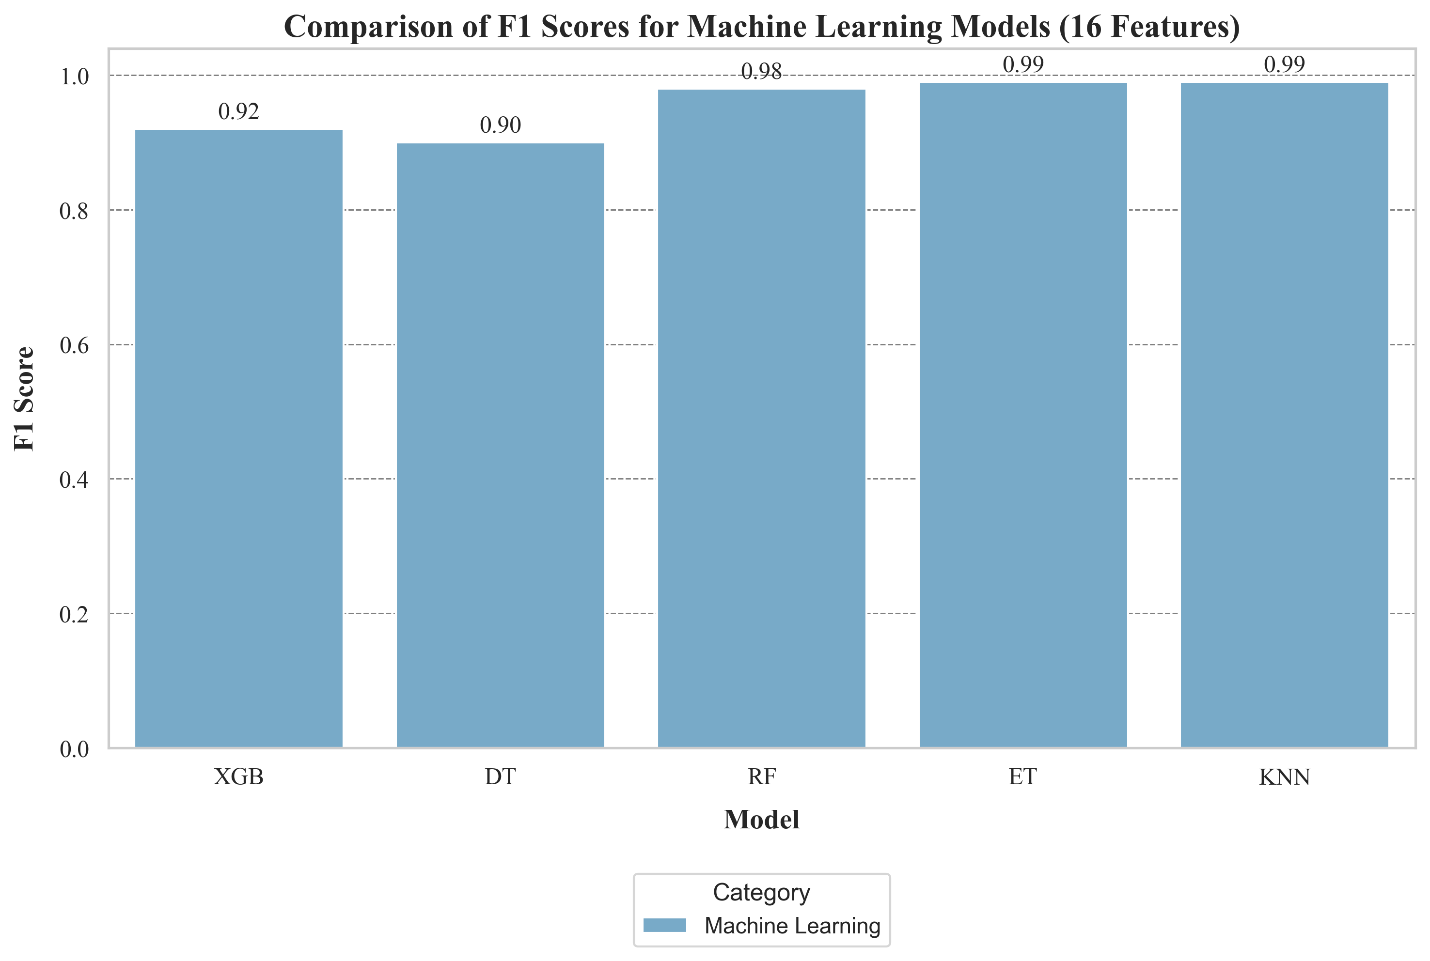
\includegraphics[width=6.4929in,height=4.3681in]{a0000-img030.png}}
\par

\bigskip

\subsubsection[Figure: Comparison of F1 Scores Across Machine Learning Models Using 16 Features]{\textbf{Figure:}
Comparison of F1 Scores Across Machine Learning Models Using 16 Features}

\bigskip


\bigskip


\bigskip


\bigskip


\bigskip


\bigskip


\bigskip


\bigskip


\bigskip


\bigskip


\bigskip


\bigskip

\subsection{Training Time Comparison Using 16 Features}
\begin{flushleft}
\tablefirsthead{}
\tablehead{}
\tabletail{}
\tablelasttail{}
\begin{supertabular}{|m{3.04206in}|m{3.04136in}|}
\hline
\centering{\bfseries Model} &
\centering\arraybslash{\bfseries Training Time (Seconds)}\\\hline
XGBoost &
\centering\arraybslash 4.59\\\hline
Decision Tree &
\centering\arraybslash 23.29\\\hline
Random Forest &
\centering\arraybslash 380.56\\\hline
Extra Trees &
\centering\arraybslash 102.52\\\hline
KNN &
\centering\arraybslash 0.04\\\hline
\end{supertabular}
\end{flushleft}

\bigskip

\centering
\lfbox[margin-right=0.0071in,margin-bottom=0.0071in,margin-top=0mm,margin-left=0mm,border-style=none,padding=0mm,vertical-align=top]{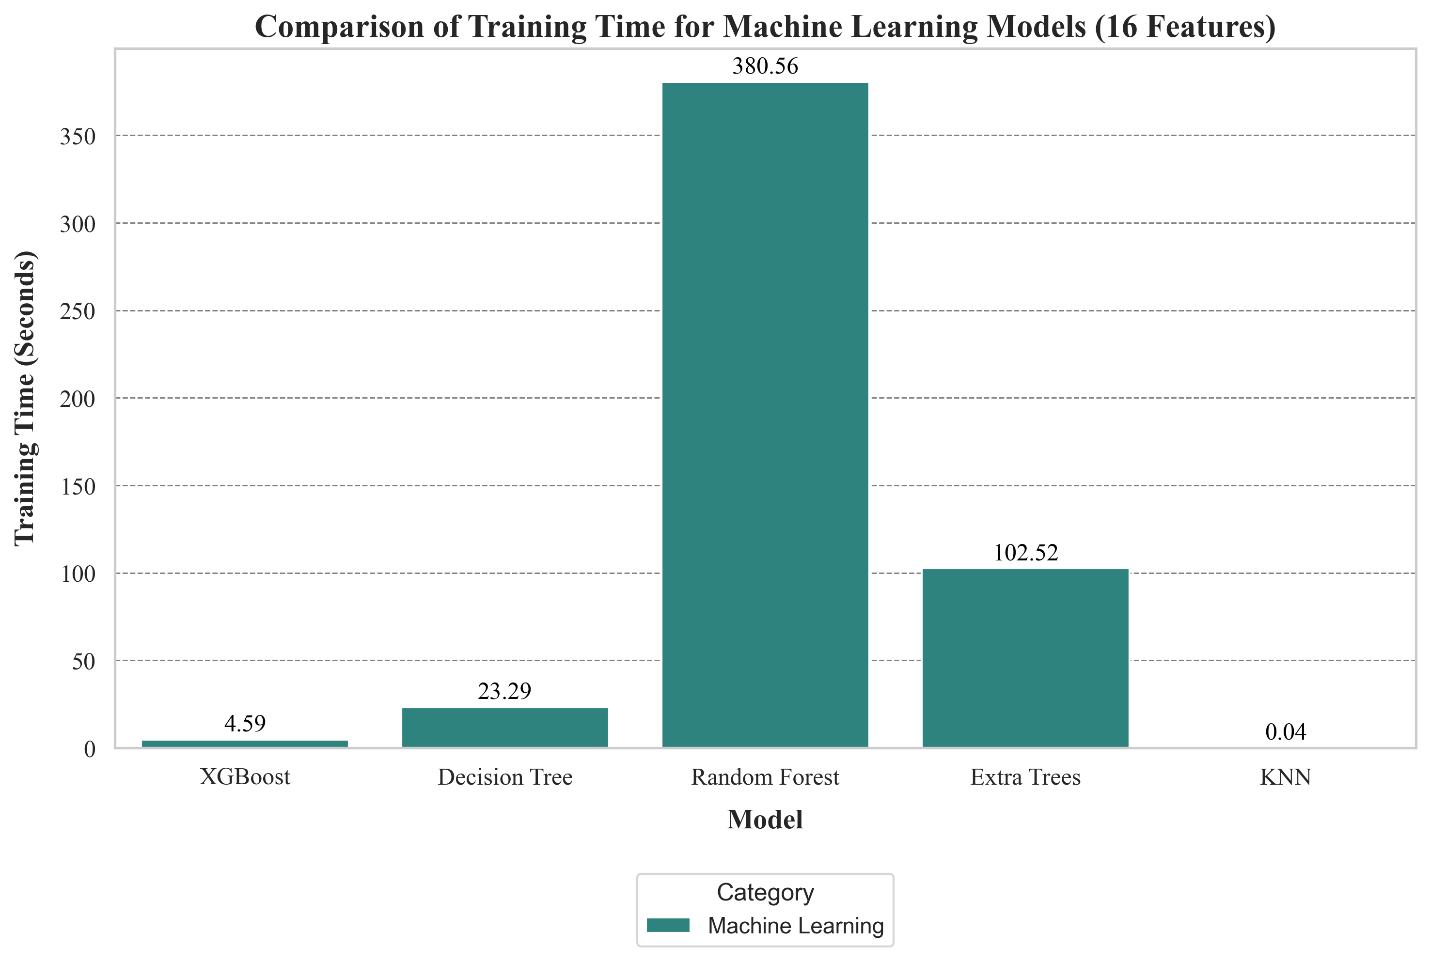
\includegraphics[width=6.4929in,height=4.3681in]{a0000-img031.png}}
\par
\subsubsection[Figure: Comparison of Training Time for Machine Learning Models Using 16 Features]{\textbf{Figure:}
Comparison of Training Time for Machine Learning Models Using 16 Features}

\bigskip


\bigskip


\bigskip


\bigskip


\bigskip

\subsection{Accuracy Comparison Using 16 Features}
\begin{flushleft}
\tablefirsthead{}
\tablehead{}
\tabletail{}
\tablelasttail{}
\begin{supertabular}{|m{2.24416in}|m{2.24486in}|m{2.24486in}|}
\hline
\centering{\bfseries Model} &
\centering{\bfseries Raw Data Accuracy} &
\centering\arraybslash{\bfseries Smoothed Data}\\\hline
XGBoost &
\centering 0.71 &
\centering\arraybslash 0.92\\\hline
Decision Tree &
\centering 0.60 &
\centering\arraybslash 0.90\\\hline
Random Forest &
\centering 0.70 &
\centering\arraybslash 0.98\\\hline
Extra Trees &
\centering 0.69 &
\centering\arraybslash 0.99\\\hline
KNN &
\centering 0.68 &
\centering\arraybslash 0.99\\\hline
\end{supertabular}
\end{flushleft}

\bigskip

\centering
\lfbox[margin-right=0.0071in,margin-top=0mm,margin-bottom=0mm,margin-left=0mm,border-style=none,padding=0mm,vertical-align=top]{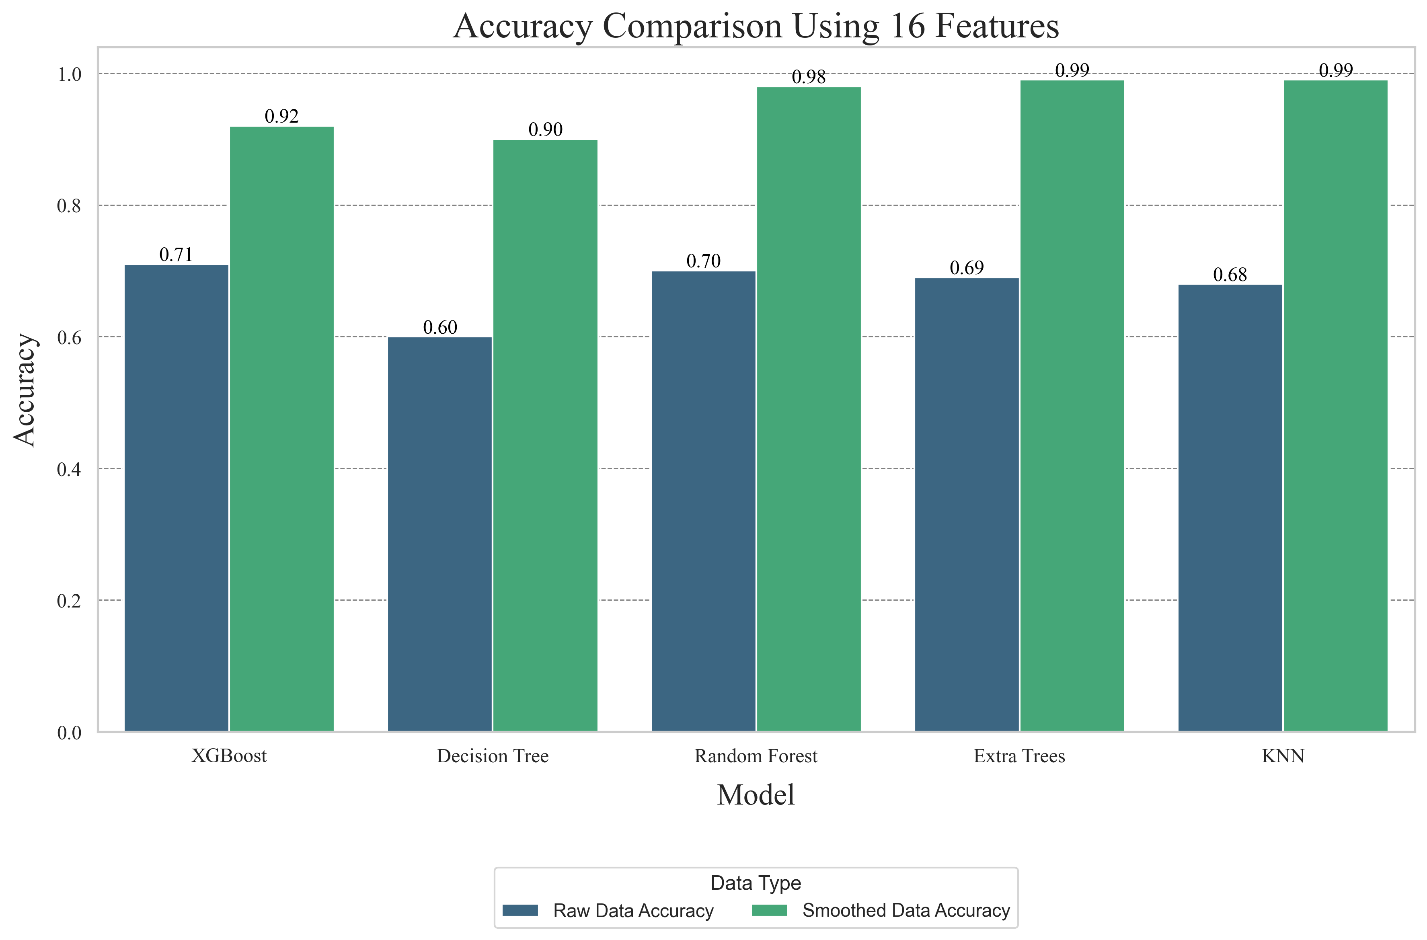
\includegraphics[width=6.4929in,height=4.278in]{a0000-img032.png}}
\par
\subsubsection[Figure: Accuracy Comparison of Machine Learning Models on Raw vs. Smoothed Data Using 16
Features]{\textbf{Figure:} Accuracy Comparison of Machine Learning Models on Raw vs. Smoothed Data Using 16 Features}

\bigskip


\bigskip


\bigskip


\bigskip

\subsection{F1 Score Comparison Using 16 Features}
\begin{flushleft}
\tablefirsthead{}
\tablehead{}
\tabletail{}
\tablelasttail{}
\begin{supertabular}{|m{2.24416in}|m{2.24486in}|m{2.24486in}|}
\hline
\centering{\bfseries Model} &
\centering{\bfseries Raw Data Accuracy} &
\centering\arraybslash{\bfseries Smoothed Data}\\\hline
XGBoost &
\centering 0.70 &
\centering\arraybslash 0.92\\\hline
Decision Tree &
\centering 0.60 &
\centering\arraybslash 0.90\\\hline
Random Forest &
\centering 0.68 &
\centering\arraybslash 0.98\\\hline
Extra Trees &
\centering 0.67 &
\centering\arraybslash 0.99\\\hline
KNN &
\centering 0.67 &
\centering\arraybslash 0.99\\\hline
\end{supertabular}
\end{flushleft}

\bigskip

\centering
\lfbox[margin-right=0.0071in,margin-top=0mm,margin-bottom=0mm,margin-left=0mm,border-style=none,padding=0mm,vertical-align=top]{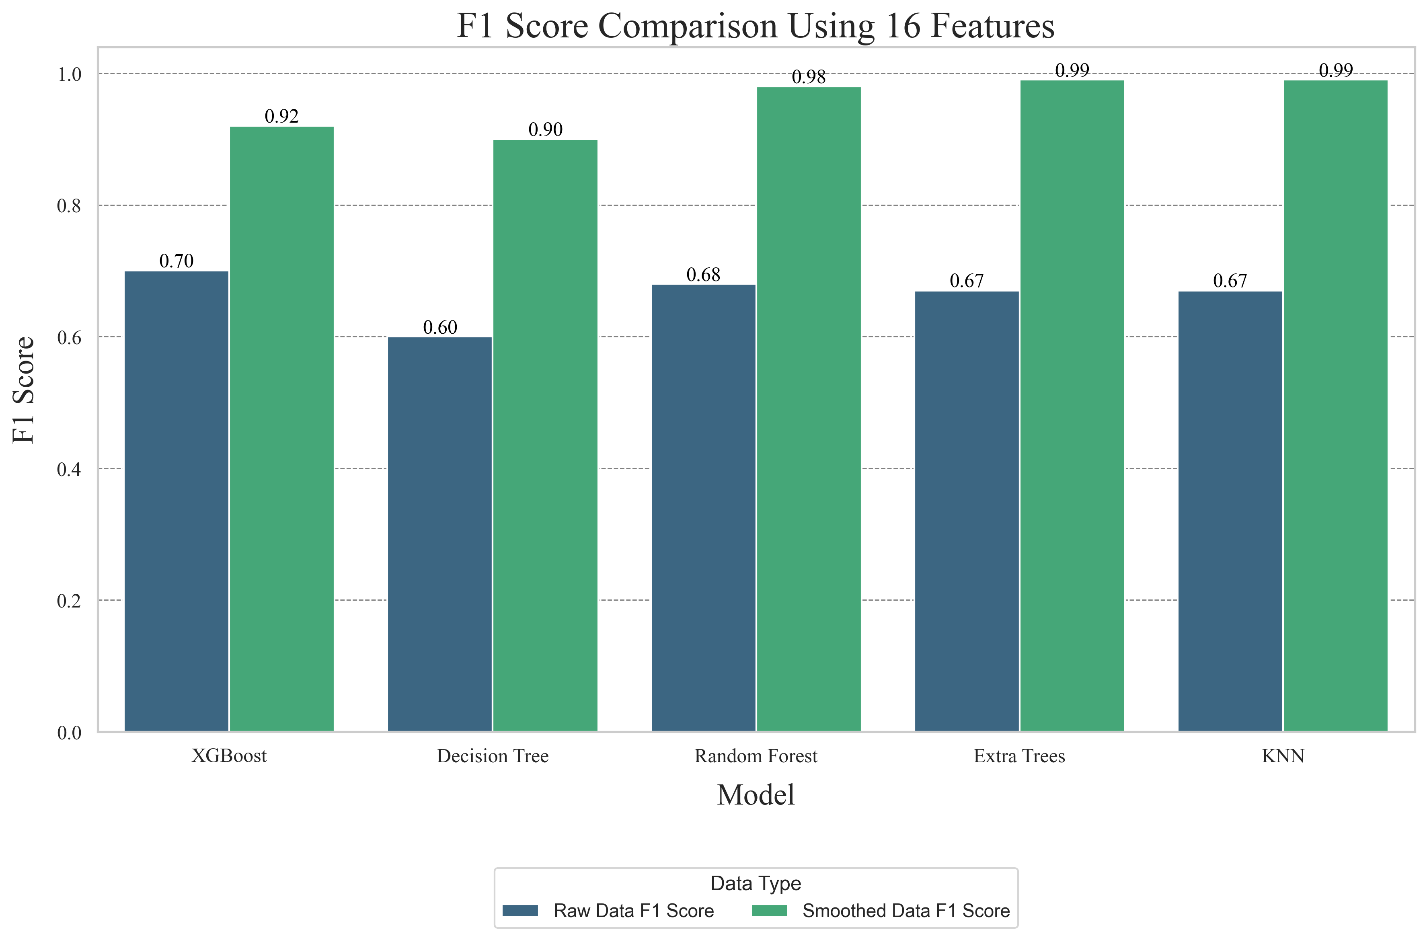
\includegraphics[width=6.4929in,height=4.278in]{a0000-img033.png}}
\par
\subsubsection[Figure: F1 Score Comparison of Machine Learning Models on Raw vs. Smoothed Data Using 16
Features]{\textbf{Figure:} F1 Score Comparison of Machine Learning Models on Raw vs. Smoothed Data Using 16 Features}

\bigskip


\bigskip


\bigskip
\end{document}
